\documentclass{article}
\usepackage{iclr2026_conference,times}

\input{math_commands.tex}

\usepackage{hyperref}
\usepackage{url}
\usepackage{amsmath}
\usepackage{amssymb}
\usepackage{graphicx}
\usepackage{subcaption}

\title{Predictive-Velocity Reward}

\author{Fangyuan Yu \\
% \texttt{fangyuan.yu18@gmail.com} \\
\And
Shuang Wu \\
\And
Xin Su \\
\And
Runyan Tan \\
\And
Phillip Howard \\
}


% Preprint mode: show real authors (via \iclrfinalcopy) and override the
% header so it does not claim conference acceptance.
\iclrfinalcopy
\begin{document}
\fancypagestyle{plain}{\fancyhf{}\lhead{Preprint. Work in progress.}\rhead{\thepage}}
\pagestyle{plain}
\lhead{Preprint. Work in progress.}


\maketitle

\begin{abstract}
Group Relative Policy Optimization (GRPO) has become the standard recipe for
reinforcement-learning fine-tuning of reasoning language models, yet it inherits
four interlocking weaknesses: long, redundant chains of thought; the absence
of a principled per-token reward; a learning-signal collapse when the base
model has near-zero pass@\(K\); and a tendency to indiscriminately penalise
every token of a failed trajectory. We propose the
\emph{predictive-velocity reward}, a dense per-token signal derived via
potential-based reward shaping from the change in answer-prediction likelihood.
The trajectory-level sum of velocities telescopes \emph{exactly} into the
\emph{information gain} contributed by the chain of thought,
\(\log p_\theta(a \mid q, o) - \log p_\theta(a \mid q)\), giving every emitted
token an explicit incentive to advance prediction of the answer. We argue that this
formulation directly mitigates redundancy, lifts the per-token signal,
and rehabilitates failed trajectories without inducing mode collapse.
\end{abstract}

\section{Introduction}

Reinforcement learning with verifiable rewards (RLVR) has driven recent
progress on coding, mathematics, and multi-step
reasoning~\citep{deepseek2025r1, kimi2025k15} by training language
models to search over long chains of thought (CoT). Much of that length
is redundant: \citet{li2025stepentropy} show that \(80\%\) of
intermediate steps can be pruned with minor accuracy loss on math
benchmarks. The wasted tokens are paid for in inference latency, in API
spend, and --- when a hard token budget is enforced --- in raw
accuracy, because rollouts get truncated before the answer is emitted.

The cause lies in how the dominant algorithm assigns credit. Group
Relative Policy Optimization (GRPO)~\citep{shao2024deepseekmath,
deepseek2025r1} and its variants~\citep{yu2025dapo, liu2025drgrpo}
grant a single sequence-level reward to each rollout from an external
verifier and use the group-relative advantage to upweight winners.
Because every token in a sequence inherits the same advantage, the
gradient cannot penalise redundant reasoning inside a successful
trajectory, nor reinforce useful sub-reasoning that happens to sit
inside a failed one. Length drift, latent-diversity collapse, and the
zero-pass@\(K\) dead zone all follow from this single coarse-grained
credit assignment (Section~\ref{sec:problem}).

What would a \emph{principled} per-token reward look like? Two
properties suffice: (i) at each step, the reward should measure how
much the emitted token advances predictability of the correct answer;
and (ii) accumulated over the trajectory, the per-token rewards should
recover a quantity that directly expresses how predictable the answer
has become given the CoT. The acid test is self-sufficiency: a
principled reward should suffice on its own to train the policy,
without being combined with an external reward through a hand-tuned
weight. Process reward
models~\citep{lightman2023letsverify, wang2024mathshepherd,
cui2025prime, setlur2024rewardingprogress} fail this test --- their
step-level scores are noisy predictions from a separately trained
verifier, are not derivable from the policy itself, and are deployed as
auxiliary regularisers stacked on top of the outcome reward.

We propose the \emph{predictive-velocity reward}, a per-token signal read
off the policy itself. The sequence-level reward is the information
gain the CoT confers on predicting the reference answer,
\(r(a, o, q) = \log p_\theta(a \mid q, o) - \log p_\theta(a \mid q)\),
and its per-token decomposition is the change in answer-prediction
log-likelihood induced by each emitted token,
\(v_t = \log p_\theta(a \mid q, o_{1:t}) - \log p_\theta(a \mid q, o_{1:t-1})\).
The \(v_t\) telescope \emph{exactly} into \(r\), so optimising the
per-token signal is a strict decomposition of an information-theoretic
objective rather than a heuristic surrogate: tokens that advance answer
prediction earn positive credit, neutral tokens earn zero, and tokens
that degrade prediction are penalised --- with no external reward model,
no length coefficient, and no change to the verifier.

\paragraph{Contributions.}
\begin{itemize}
  \item We trace four interlocking GRPO pathologies --- CoT
        redundancy, the absence of a per-token signal, the
        zero-pass@\(K\) dead zone, and indiscriminate trajectory-level
        credit --- to a single cause, the sparse outcome reward
        (Section~\ref{sec:problem}).
  \item We define the \emph{predictive-velocity reward}, the unique
        per-token decomposition of CoT information gain, computable
        from the policy alone (Section~\ref{sec:method}).
  \item We complement the reward with an \emph{answer buffer} and a
        \emph{prefix buffer} --- diversifying the target the CoT is
        graded against and the starting point from which it is built
        --- and a \emph{per-token advantage} rule that favours the
        shortest trajectory among those of maximum information gain.
  \item On Game of 24 across \(\{0.6,1.7,4\}\)B model scales and
        \(\{512,1024\}\)-token CoT budgets we document the baseline
        GRPO pathologies the method targets and establish the
        diagnostic battery on which it will be evaluated
        (Section~\ref{subsec:baseline-diag}).
\end{itemize}

\section{The Four Drawbacks of GRPO}
\label{sec:problem}

\paragraph{(D1) CoT redundancy.}
Reasoning models routinely emit thousands of CoT tokens for problems that, in
principle, require only a few. Much of the chain is filler that neither
constrains the answer distribution nor verifies intermediate computation:
\citet{li2025stepentropy} show that on math benchmarks across DeepSeek-R1-7B,
14B and Qwen3-8B, roughly \(80\%\) of \emph{low-entropy} intermediate
reasoning steps can be pruned with only minor accuracy loss, while random or
high-entropy pruning collapses performance --- a direct empirical lower bound
on how much of the chain is informationally redundant.
Practitioners have addressed this with explicit length penalties or
short-answer bonuses, but such auxiliary rewards are fundamentally
unprincipled: a hand-tuned length term is a separate objective bolted onto the
correctness reward and almost always trades against accuracy, forcing
brittle coefficient sweeps to balance the two. What is missing is a
\emph{single} reward whose structure already prices the cost of additional
tokens against their contribution to solving the problem.

\paragraph{(D2) No principled per-token signal.}
The reward in GRPO is sparse and trajectory-level. Every intermediate token
inherits the same advantage estimate, leaving the per-token credit assignment
uncalibrated and the gradient noisy.

\paragraph{(D3) The zero-pass@\(K\) dead zone.}
When the base model has near-zero pass@\(K\) on a task, the group of sampled
trajectories contains no positives, the relative advantage collapses to zero,
and the policy receives no learning signal. The model never lifts off such
tasks.

\paragraph{(D4) Indiscriminate credit assignment.}
GRPO discriminates against \emph{every} token in a failed trajectory and
accepts \emph{every} token in a successful one, regardless of whether that
token was actually responsible for the outcome. This invites mode collapse,
discards genuinely useful sub-trajectories that happened to terminate badly,
reinforces filler tokens that happened to ride along with success, and is a
poor model of how credit propagates through reasoning.

\section{Method: Predictive-Velocity Reward}
\label{sec:method}

\subsection{Setup and Notation}

Let \(q\) denote a query, \(o = (o_1, o_2, \dots, o_T)\) a chain-of-thought
sequence generated by the policy, and \(a\) the answer. The policy is the
language model \(p_\theta\). We assume access to a reference answer \(a\) per
query (e.g.\ a gold answer; the formulation extends to a set of equivalent
answers by taking an expectation).

\subsection{Sequence-Level: Information-Gain Reward}

We define the sequence-level CoT reward as the \emph{information gain} of the
answer under the policy when the CoT is conditioned on, relative to the
direct-answer baseline:
\begin{equation}
r(a, o, q)
\;:=\;
\log p_\theta(a \mid q, o) \;-\; \log p_\theta(a \mid q).
\label{eq:rseq}
\end{equation}
Adopting the convention \(r(a, q) := \log p_\theta(a \mid q)\) for the
no-CoT case, \(r(a, o, q)\) measures \emph{how much the CoT helps} the policy
predict the answer. This is a more principled target than the raw answer-prediction
likelihood \(\log p_\theta(a \mid q, o)\): the latter is satisfied by any
prefix that merely \emph{correlates} with \(a\), whereas
Equation~\ref{eq:rseq} rewards the CoT's \emph{causal contribution} (Section~\ref{subsec:buys}).

\subsection{Token-Level: Velocity Reward}

For each token \(o_t\), we define the \emph{velocity reward} as the change in
sequence-level reward induced by emitting that token:
\begin{equation}
v(a, o_{1:t}, q)
\;:=\;
r(a, o_{1:t}, q) - r(a, o_{1:t-1}, q)
\;=\;
\log p_\theta(a \mid q, o_{1:t}) - \log p_\theta(a \mid q, o_{1:t-1}).
\label{eq:rvel}
\end{equation}
By telescoping, the trajectory return equals the sequence-level reward
exactly:
\begin{equation}
\sum_{t=1}^{T} v(a, o_{1:t}, q)
\;=\;
\sum_{t=1}^{T} \bigl[ r(a, o_{1:t}, q) - r(a, o_{1:t-1}, q) \bigr]
\;=\;
r(a, o, q).
\label{eq:telescope}
\end{equation}
\textbf{Equivalence.}  Equation~\ref{eq:telescope} establishes that
\emph{optimising the per-token velocity reward is exactly equivalent, at the
trajectory level, to optimising the information gain contributed by the
CoT.} No bound, no approximation, no shaping coefficient.

\subsection{Online Answer Buffer}
\label{subsec:buffer}

The formulation so far conditions on a single reference answer \(a\), but
many queries admit \emph{multiple} correct answers -- numerically equivalent
expressions, equivalent code, or paraphrastic restatements. Optimising
against a single \(a\) risks overfitting the CoT to a specific surface form
of the correct answer rather than to the underlying solution.

We therefore maintain an \emph{online answer buffer} \(\mathcal{A}_q\) per
query, populated by all correct answers the policy has produced so far, as
judged by the verifiable reward function:
\begin{equation}
\mathcal{A}_q \;:=\; \{a \mid a \text{ is a correct answer for } q\}.
\label{eq:buffer}
\end{equation}
At training time we sample \(a \sim \mathrm{unif}(\mathcal{A}_q)\) when
evaluating the information-gain reward, replacing
\(\log p_\theta(a \mid q, o)\) in Equations~\ref{eq:rseq} and \ref{eq:rvel}
with
\(\mathbb{E}_{a \sim \mathrm{unif}(\mathcal{A}_q)}\!\bigl[\log p_\theta(a \mid q, o)\bigr]\).
This encourages the policy to learn a \emph{general} CoT that predicts the
class of correct answers, rather than overfitting to any one of them. The
buffer is built online from the model's own successful rollouts and grows
monotonically over training; until a query has at least one entry in
\(\mathcal{A}_q\), we fall back to the gold reference answer.

\subsection{Online Prefix Buffer}
\label{subsec:prefix}

Symmetric to the answer buffer of Section~\ref{subsec:buffer}, we maintain a
\emph{prefix buffer} \(\mathcal{P}_q\) per query, recording CoT prefixes the
model has produced so far that score highly under the answer-prediction objective
\emph{relative to other prefixes of the same length}:
\begin{equation}
\mathcal{P}_q \;:=\; \{\, o_{1:t} \;\mid\; 1 \le t < T \,\},
\label{eq:prefix-buffer}
\end{equation}
organised as a priority queue. Concretely, we bin prefixes by length \(t\)
and, within each bin, retain the top-\(K\) prefixes ranked by the cumulative
velocity reward
\(\sum_{s \le t} v(a, o_{1:s}, q) = \log p_\theta(a \mid q, o_{1:t}) - \log p_\theta(a \mid q)\)
-- i.e.\ the partial information gain achieved by the prefix.

During rollout, we occasionally seed the policy with a sampled prefix from
\(\mathcal{P}_q\) and let it continue from there. This serves two purposes:
(i)~it amortises the cost of rediscovering productive CoT openings, and
(ii)~it injects exploration around \emph{known-good} subsequences without
discarding the benefits of unconstrained sampling. Together with the answer
buffer, the two structures form a complementary memory: \(\mathcal{A}_q\)
diversifies the \emph{target} the CoT is graded against, \(\mathcal{P}_q\)
diversifies the \emph{starting point} from which the CoT is built.

\subsection{Per-Token Advantage}
\label{subsec:advantage}

GRPO computes a single advantage per trajectory and broadcasts it to every
token. With a genuinely per-token reward in hand, we compute a per-token
advantage instead. The challenge is that rollouts in a group have different
CoT lengths, so per-position statistics are not directly comparable.

Consider a group of \(N\) rollouts with per-token velocity rewards
\[
\bigl\{\,
(o^{i}_{1:T_i}, v^{i}_{1:T_i}) \,\bigr\}_{i=1}^{N},
\qquad
v^{i}_{t} \;:=\; v(a, o^{i}_{1:t}, q).
\]
We truncate the CoT sequence of every rollout to a common length \(T^{*}\) defined as
\emph{the shortest length among rollouts that achieve the highest
trajectory-level information gain}:
\begin{equation}
T^{*}
\;:=\;
\min \!\left\{\, T_i \;\Big|\; i \in \arg\max_{j} \sum_{t=1}^{T_j} v^{j}_{t} \,\right\}.
\label{eq:tstar}
\end{equation}
After truncation, every rollout's CoT has length \(T^{*}\) and per-position
advantages can be computed by standard group-relative normalisation across
the \(N\) rollouts at each \(t \in \{1, \dots, T^{*}\}\).

\textbf{Why this rule.} The truncation policy explicitly favours the
\emph{shortest} winner: among all trajectories that achieve the maximum
trajectory return, it selects the most concise. Rollouts longer than
\(T^{*}\) have their tail tokens dropped from the loss, so a longer
trajectory is preferred only if it strictly improves the trajectory return.
This realises the ``length and accuracy in one signal'' property of D1 at
the level of credit assignment: redundant tokens past \(T^{*}\) receive
neither reward nor advantage, and shorter, denser CoTs become the implicit
target of optimisation.

\subsection{What This Buys Us}
\label{subsec:buys}

\paragraph{D1 -- CoT redundancy is priced at every scale.}

\paragraph{D2 -- Per-token rewards accumulate to the predictive
likelihood.} By Equation~\ref{eq:telescope}, the per-token velocities
sum exactly to \(\log p_\theta(a \mid q, o) - \log p_\theta(a \mid q)\)
--- the gain in answer predictability conferred by the CoT. The
per-token signal is therefore principled by construction: it is not a
heuristic surrogate but the unique decomposition of an
information-theoretic, policy-internal target.

\paragraph{D3 -- Learning from failure trajectories.}

\paragraph{D4 -- Explicit diversity encouragement via prefix and answer
caching.} The answer buffer \(\mathcal{A}_q\)
(Section~\ref{subsec:buffer}) and the prefix buffer \(\mathcal{P}_q\)
(Section~\ref{subsec:prefix}) diversify, respectively, the target the
CoT is graded against and the starting point from which it is built;
together they act as an explicit anti-mode-collapse pressure on top of
the velocity reward.

\section{Experiments}
\label{sec:exp}

\textit{This section is under active development.} We outline below the
experiments that will populate this section.

\subsection{Research Questions}
\label{subsec:rq}

The Experiments section is organised around three head-to-head comparisons
between vanilla GRPO and GRPO augmented with the predictive-velocity reward
(plus the answer buffer \(\mathcal{A}_q\) and prefix buffer \(\mathcal{P}_q\)
of Section~\ref{sec:method}). Each question targets one of the drawbacks
that the method is designed to address.

\begin{itemize}
  \item \textbf{(RQ1, targets D1)} Does the velocity reward shorten the
        CoT without hurting accuracy under a matched \(T_{\max}\)?
  \item \textbf{(RQ2, targets D3)} Does it break the zero-pass@\(K\)
        dead zone, where vanilla GRPO has no positive trajectory to
        reweight?
  \item \textbf{(RQ3, targets the prefix buffer)} Does
        \(\mathcal{P}_q\) raise the number of distinct correct
        solutions per puzzle relative to vanilla GRPO?
\end{itemize}

\subsection{Baseline GRPO diagnostics on Game of 24}
\label{subsec:baseline-diag}

Before reporting velocity-reward results we characterise what
\emph{vanilla} GRPO does on Game of 24, swept across model scale
\(\{\text{Qwen3-0.6B},\,\text{Qwen3-1.7B},\,\text{Qwen3-4B}\}\) and CoT
budget \(T_{\max}\in\{512,\,1024\}\). All six runs share the same prompt
template, verifier (an expression evaluator that accepts any parenthesised
arithmetic expression over the four input digits that evaluates to 24),
group size \(G=8\), and 1200 GRPO update steps. Evaluation is performed
every 200 steps on a held-out set of 84 puzzles, sampling \(G\) rollouts
per puzzle; the diagnostics below are computed at the final step. Visual
encoding is consistent across panels: \emph{colour} encodes model size
(0.6B blue, 1.7B teal, 4B red) and \emph{linestyle} encodes budget (solid
\(=512\), dashed \(=1024\)).

These diagnostics serve three purposes: (i) they make the redundancy
that motivates D1 (Section~\ref{sec:problem}) concrete on a controlled
task --- truncation pressure at small budgets and per-cycle CoT-length
drift; (ii) they establish a battery of measurement tools --- per-cycle
solution coverage, within-puzzle prefix collapse, predictive-velocity
correctness contrast --- that we will reuse when reporting
velocity-reward results; and (iii) they expose the failure modes the
method must improve upon.

\paragraph{Truncation and accuracy (K1, Fig.~\ref{fig:k1}).}
Accuracy rises with both model size and budget, except at
\(T_{\max}=512\) where 0.6B and 1.7B tie at 0.408 because both saturate
the budget.

\begin{figure}[t]
  \centering
  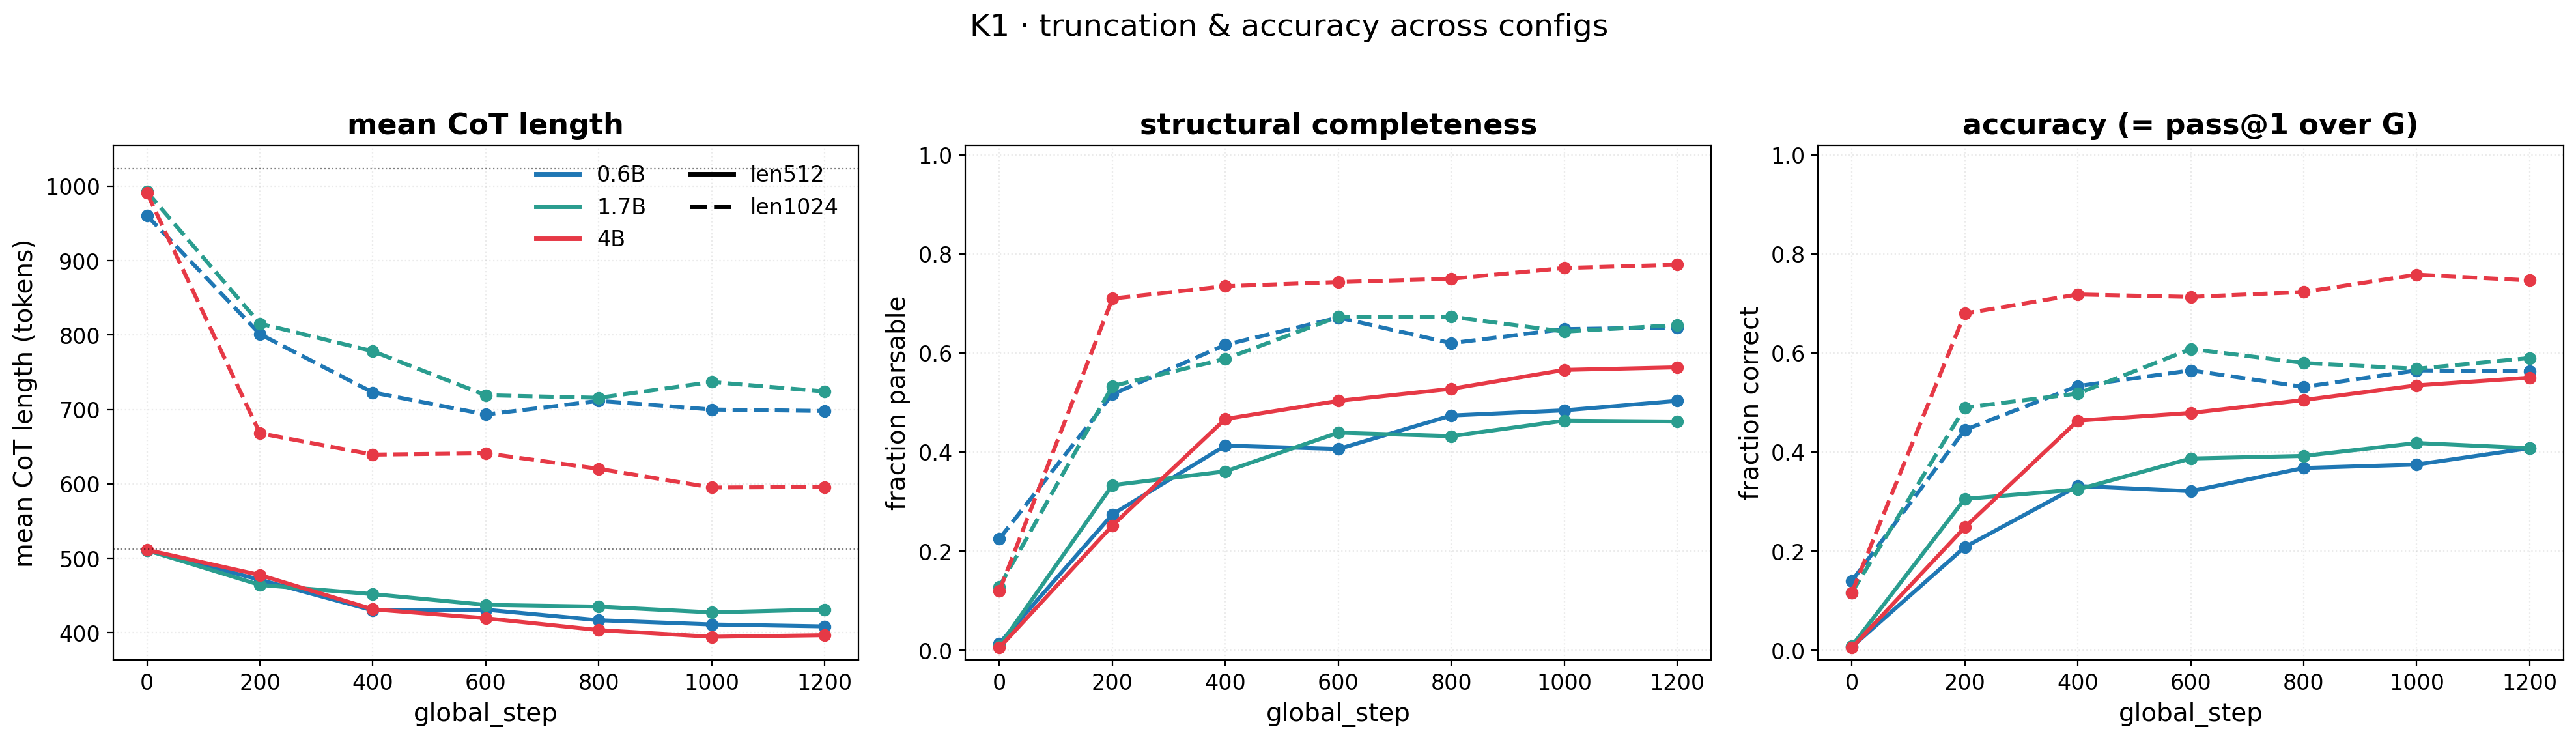
\includegraphics[width=\linewidth]{figures/game24-k1.png}
  \caption{\textbf{K1 --- Truncation and accuracy.} Mean CoT length
  (left), structural completeness (centre), and accuracy (right) across
  GRPO updates for each (model, budget). Dotted horizontals mark
  \(T_{\max}\). All curves are averaged over 84 held-out puzzles \(\times\)
  \(G=8\) rollouts.}
  \label{fig:k1}
\end{figure}

\paragraph{Length split by correctness, and within-puzzle diversity (K2,
Fig.~\ref{fig:k2}).}
Stronger models need shorter CoTs to succeed, and within-puzzle
diversity grows when the budget is lifted from 512 to 1024.

\begin{figure}[t]
  \centering
  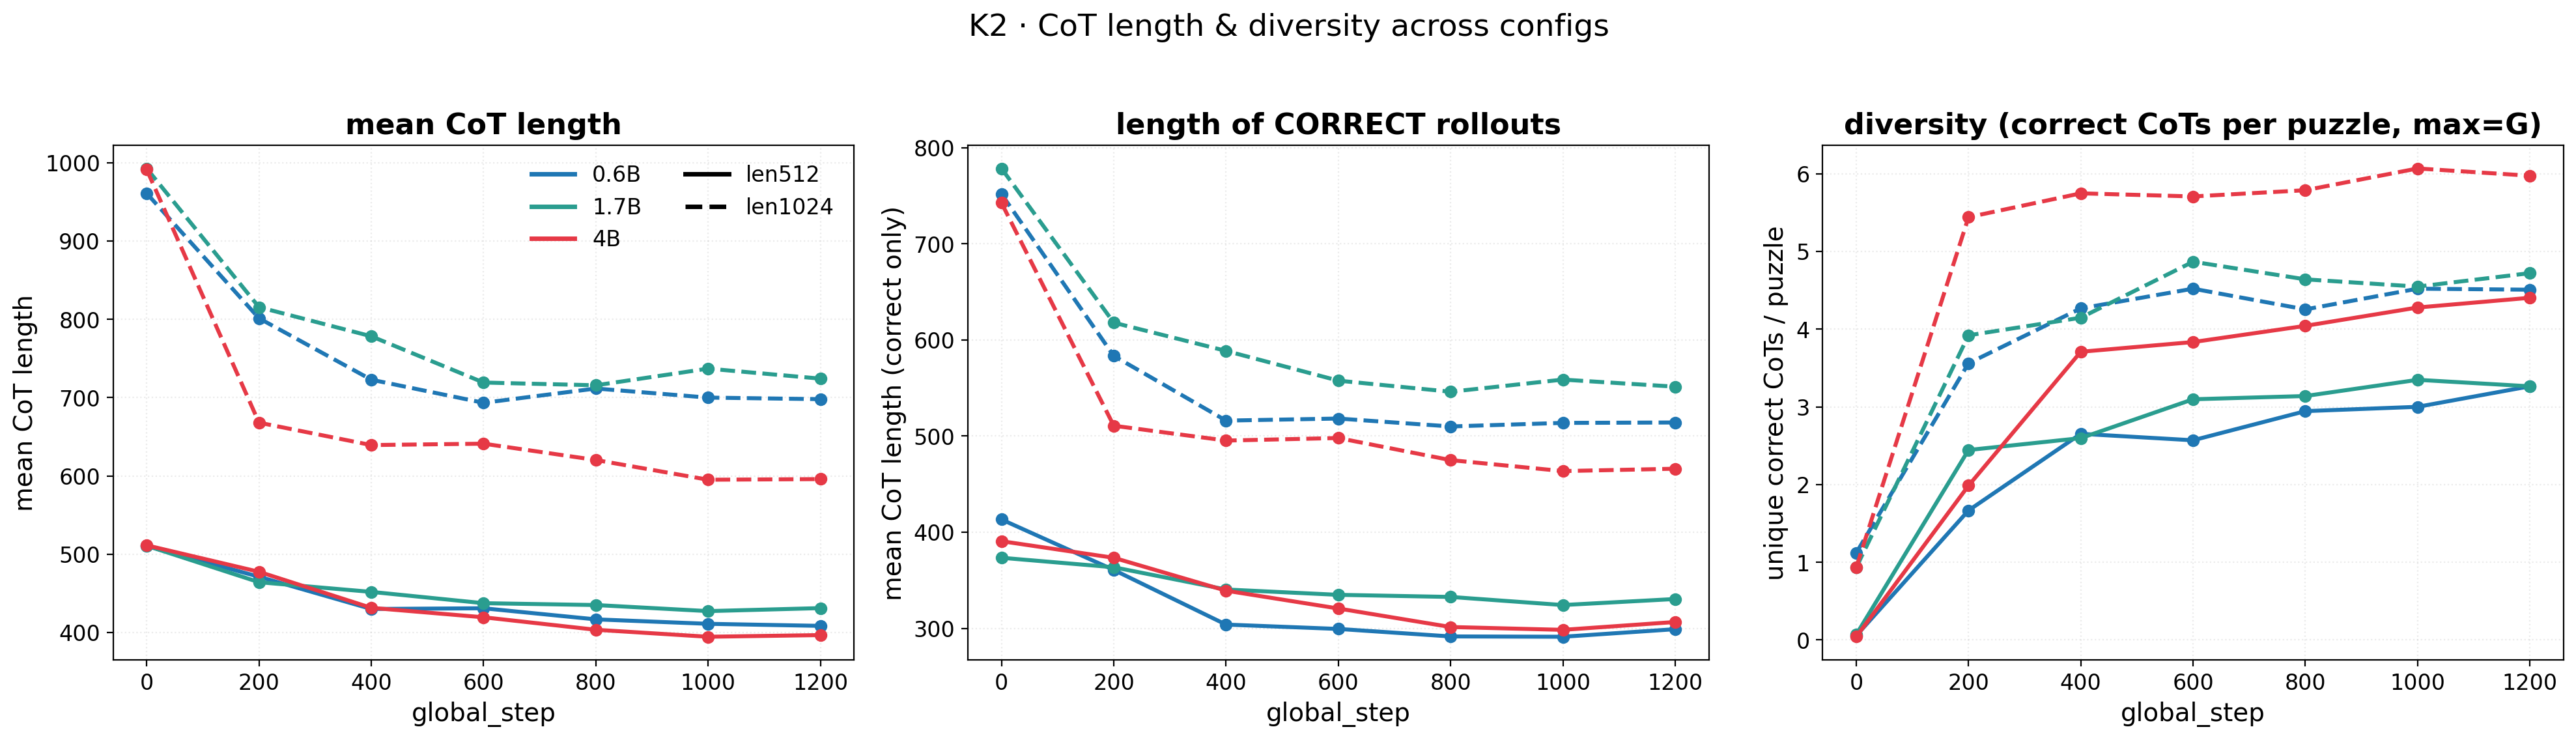
\includegraphics[width=\linewidth]{figures/game24-k2.png}
  \caption{\textbf{K2 --- CoT length and diversity.} Mean CoT length
  (left), mean length of \emph{correct} rollouts only (centre), and
  unique correct CoTs per puzzle out of \(G=8\) (right).}
  \label{fig:k2}
\end{figure}

\paragraph{pass@1 and pass@8 (K3, Fig.~\ref{fig:k3}).}
The pass@8\(-\)pass@1 gap shrinks with model size --- larger models
concentrate on fewer solution templates, the empirical target for the
prefix buffer \(\mathcal{P}_q\) (RQ3).

\begin{figure}[t]
  \centering
  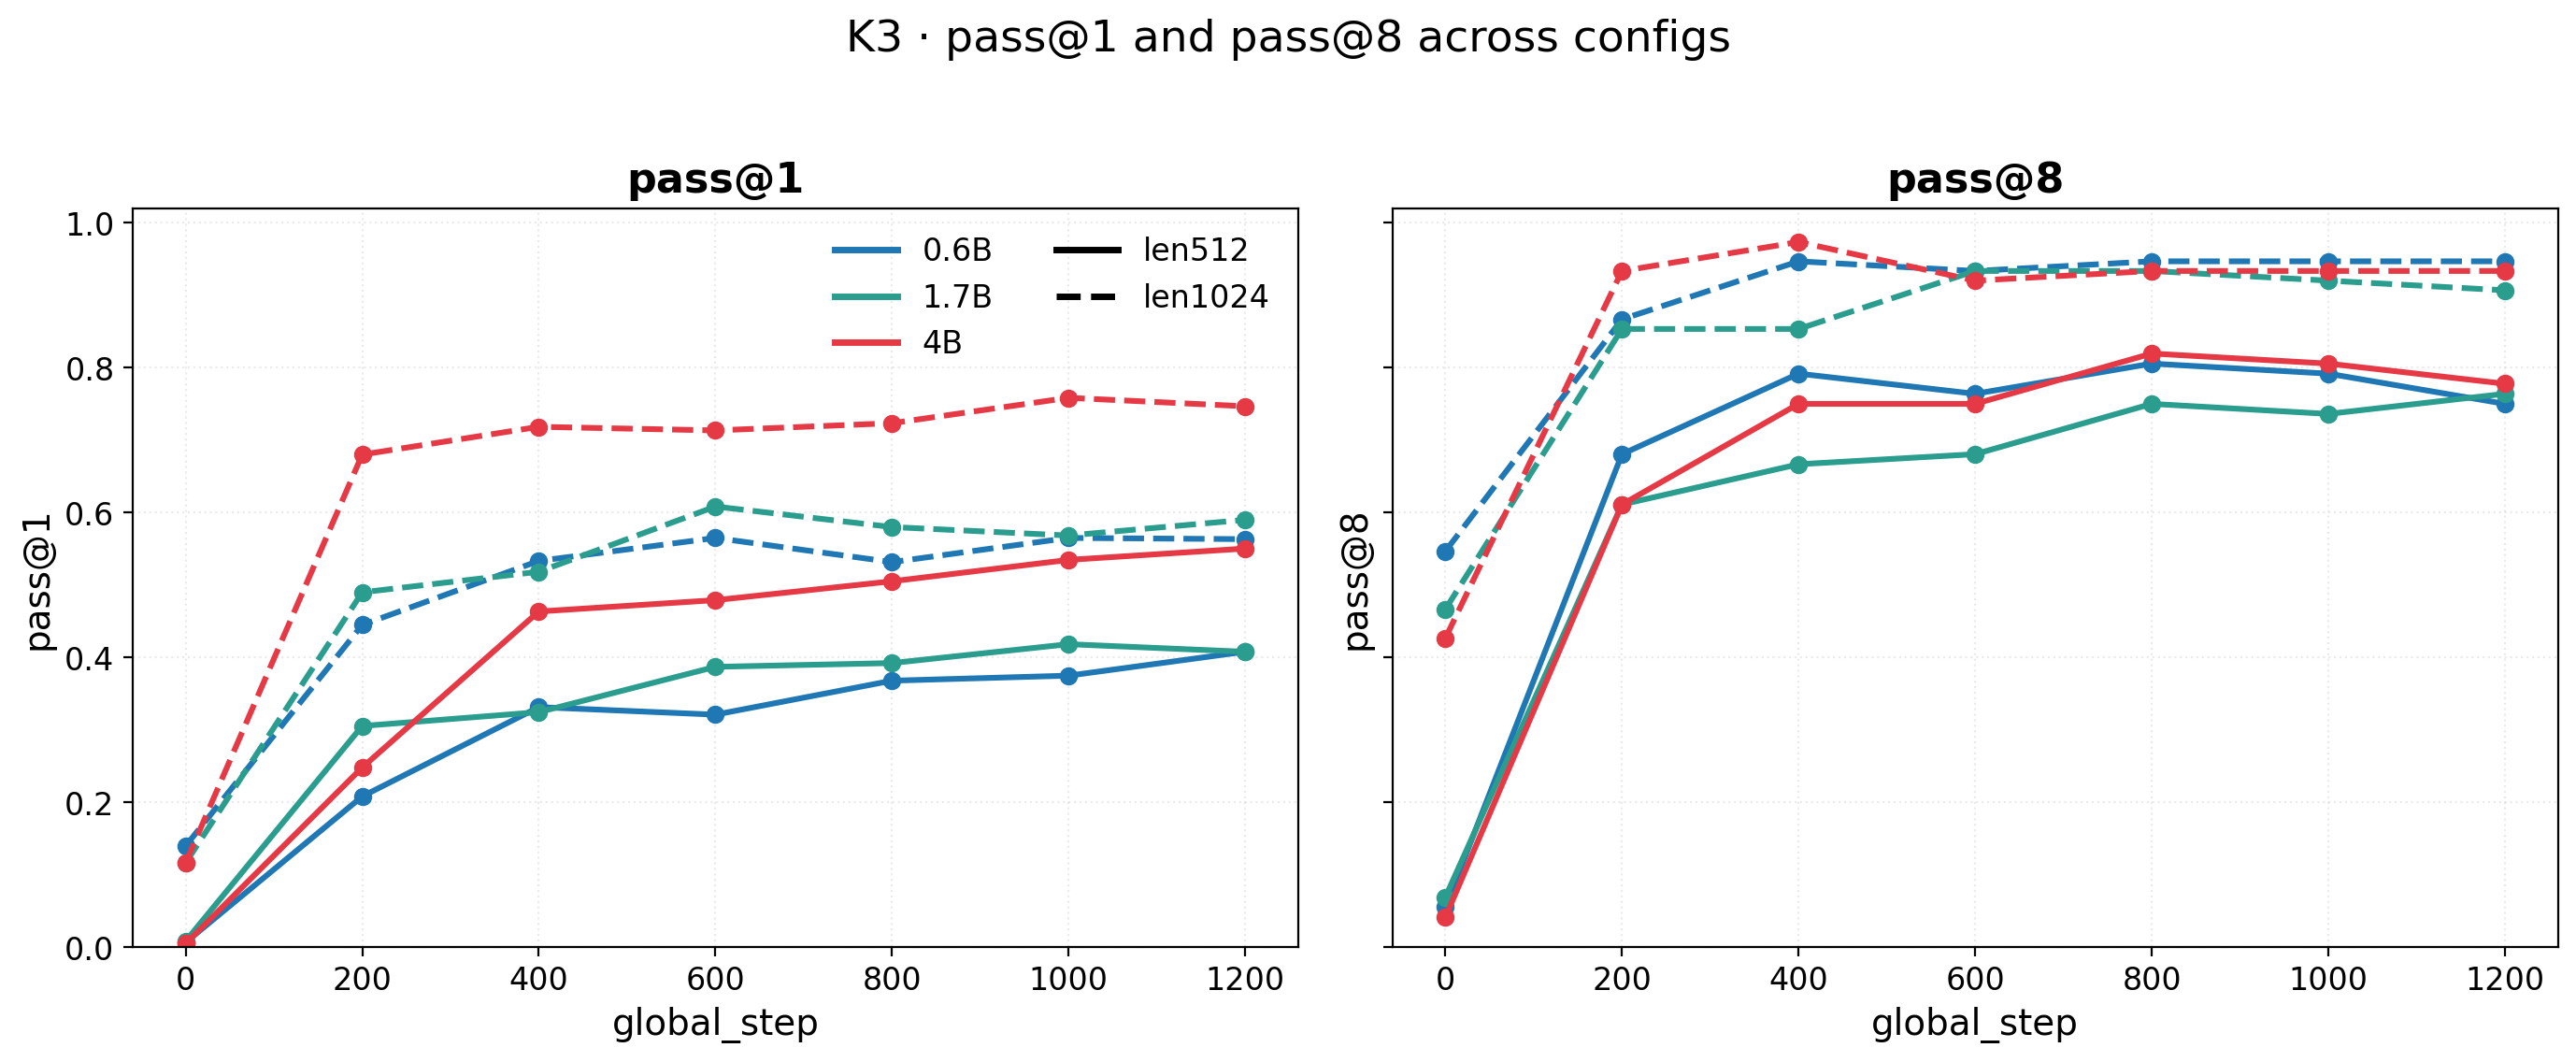
\includegraphics[width=\linewidth]{figures/game24-k3.png}
  \caption{\textbf{K3 --- pass@1 and pass@8.} pass@8 \(-\) pass@1 quantifies
  the head-room left by single-shot sampling.}
  \label{fig:k3}
\end{figure}

\paragraph{Solution-coverage dynamics (K4, Fig.~\ref{fig:k4}).}
Solution coverage is overall poor: cumulative coverage saturates below
\(25\%\) of canonical solutions for every config, only about a third of
the \(G\) rollouts emit distinct solutions in any given cycle, and the
novel fraction monotonically declines from step 200 onwards --- the
mode collapse that motivates \(\mathcal{P}_q\).

\begin{figure}[t]
  \centering
  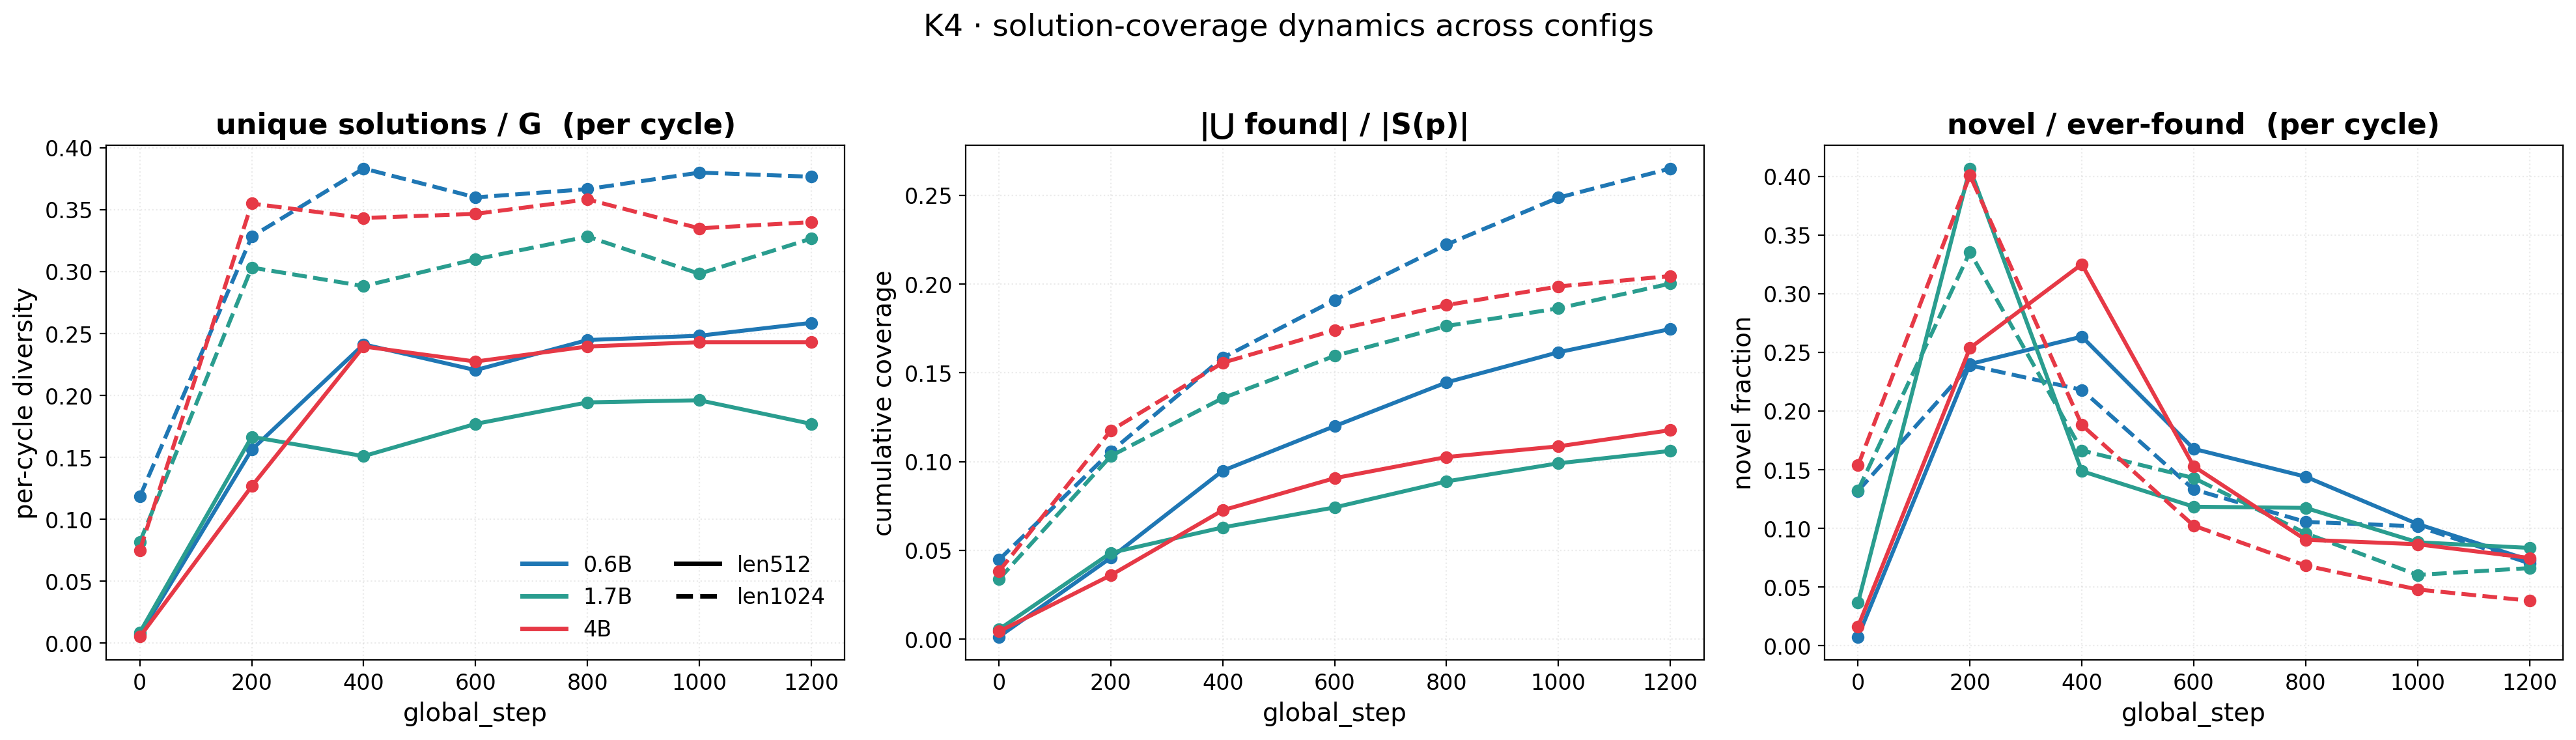
\includegraphics[width=\linewidth]{figures/game24-k4.png}
  \caption{\textbf{K4 --- Solution-coverage dynamics.} Per-cycle diversity
  (left), cumulative coverage of canonical \(=24\) solutions (centre),
  and per-cycle novel fraction (right).}
  \label{fig:k4}
\end{figure}

\paragraph{Within-puzzle prefix collapse (K5, Fig.~\ref{fig:k5}).}
At the other end of a rollout, heavy within-puzzle prefix sharing is
observed: top-1 prefix share falls with model size and budget but
every config stays far above the \(1/G=0.125\) floor of an uncollapsed
policy.

\begin{figure}[t]
  \centering
  \begin{subfigure}[t]{0.55\linewidth}
    \centering
    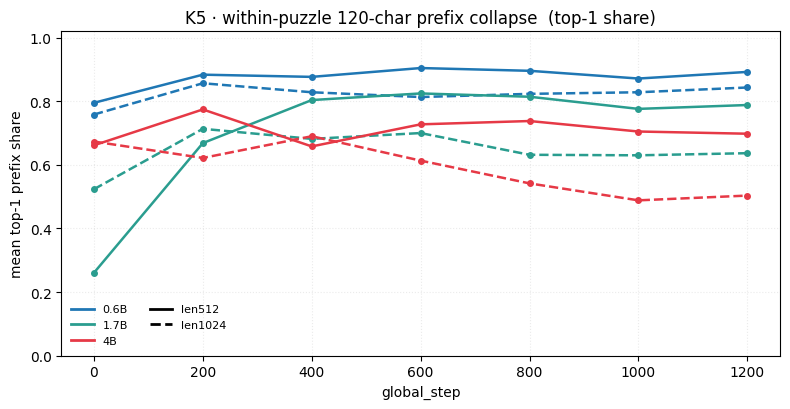
\includegraphics[width=\linewidth]{figures/game24-k5.png}
    \caption{\textbf{K5 --- Within-puzzle 120-character prefix collapse.}
    Mean fraction of the \(G\) rollouts for a puzzle that share the
    most-common 120-character CoT prefix. Higher \(=\) more
    prefix-collapsed.}
    \label{fig:k5}
  \end{subfigure}\hfill
  \begin{subfigure}[t]{0.43\linewidth}
    \centering
    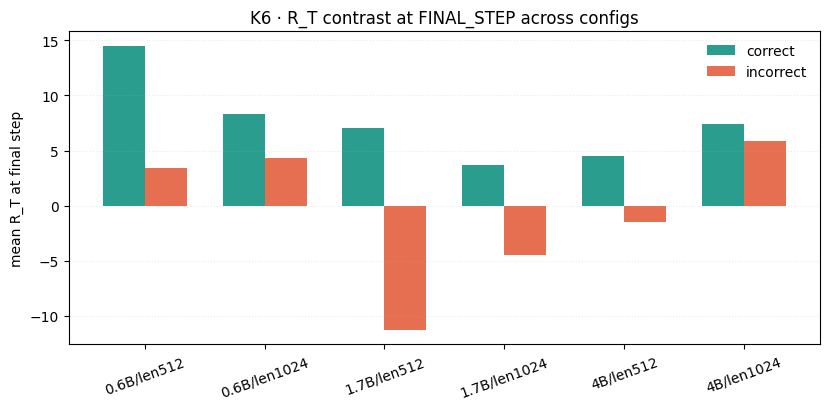
\includegraphics[width=\linewidth]{figures/game24-k6.png}
    \caption{\textbf{K6 --- Predictive-velocity correctness contrast at the
    final step.} Mean \(R_T\) of correct (green) vs. incorrect (orange)
    rollouts per configuration. Correct rollouts are scored against
    their own emitted expression; incorrect rollouts against the
    best-matching canonical \(=24\)-solution.}
    \label{fig:k6}
  \end{subfigure}
  \caption{K5 and K6 diagnostics at the final GRPO step.}
  \label{fig:k5k6}
\end{figure}

\paragraph{Predictive-velocity correctness contrast (K6,
Fig.~\ref{fig:k6}).}
\(R_T\) is generally a useful signal that separates correct from
incorrect rollouts; the gap shrinks as the policy gets stronger, where
\(R_T\) acts mainly as a compaction pressure (RQ1) rather than as a
discriminator.

\paragraph{Per-prefix-position correctness contrast (K7,
Fig.~\ref{fig:k7}).}
The within-puzzle \(\Delta R_t = \overline{R_t}_{\text{correct}} -
\overline{R_t}_{\text{incorrect}}\) curves are dominated by late-CoT
tokens (\(\tau \gtrsim 0.7\)); at smaller scales and tighter budgets
the early-CoT contrast dips sharply negative before recovering --- the
temporal signature of the K5 prefix collapse.

\begin{figure}[t]
  \centering
  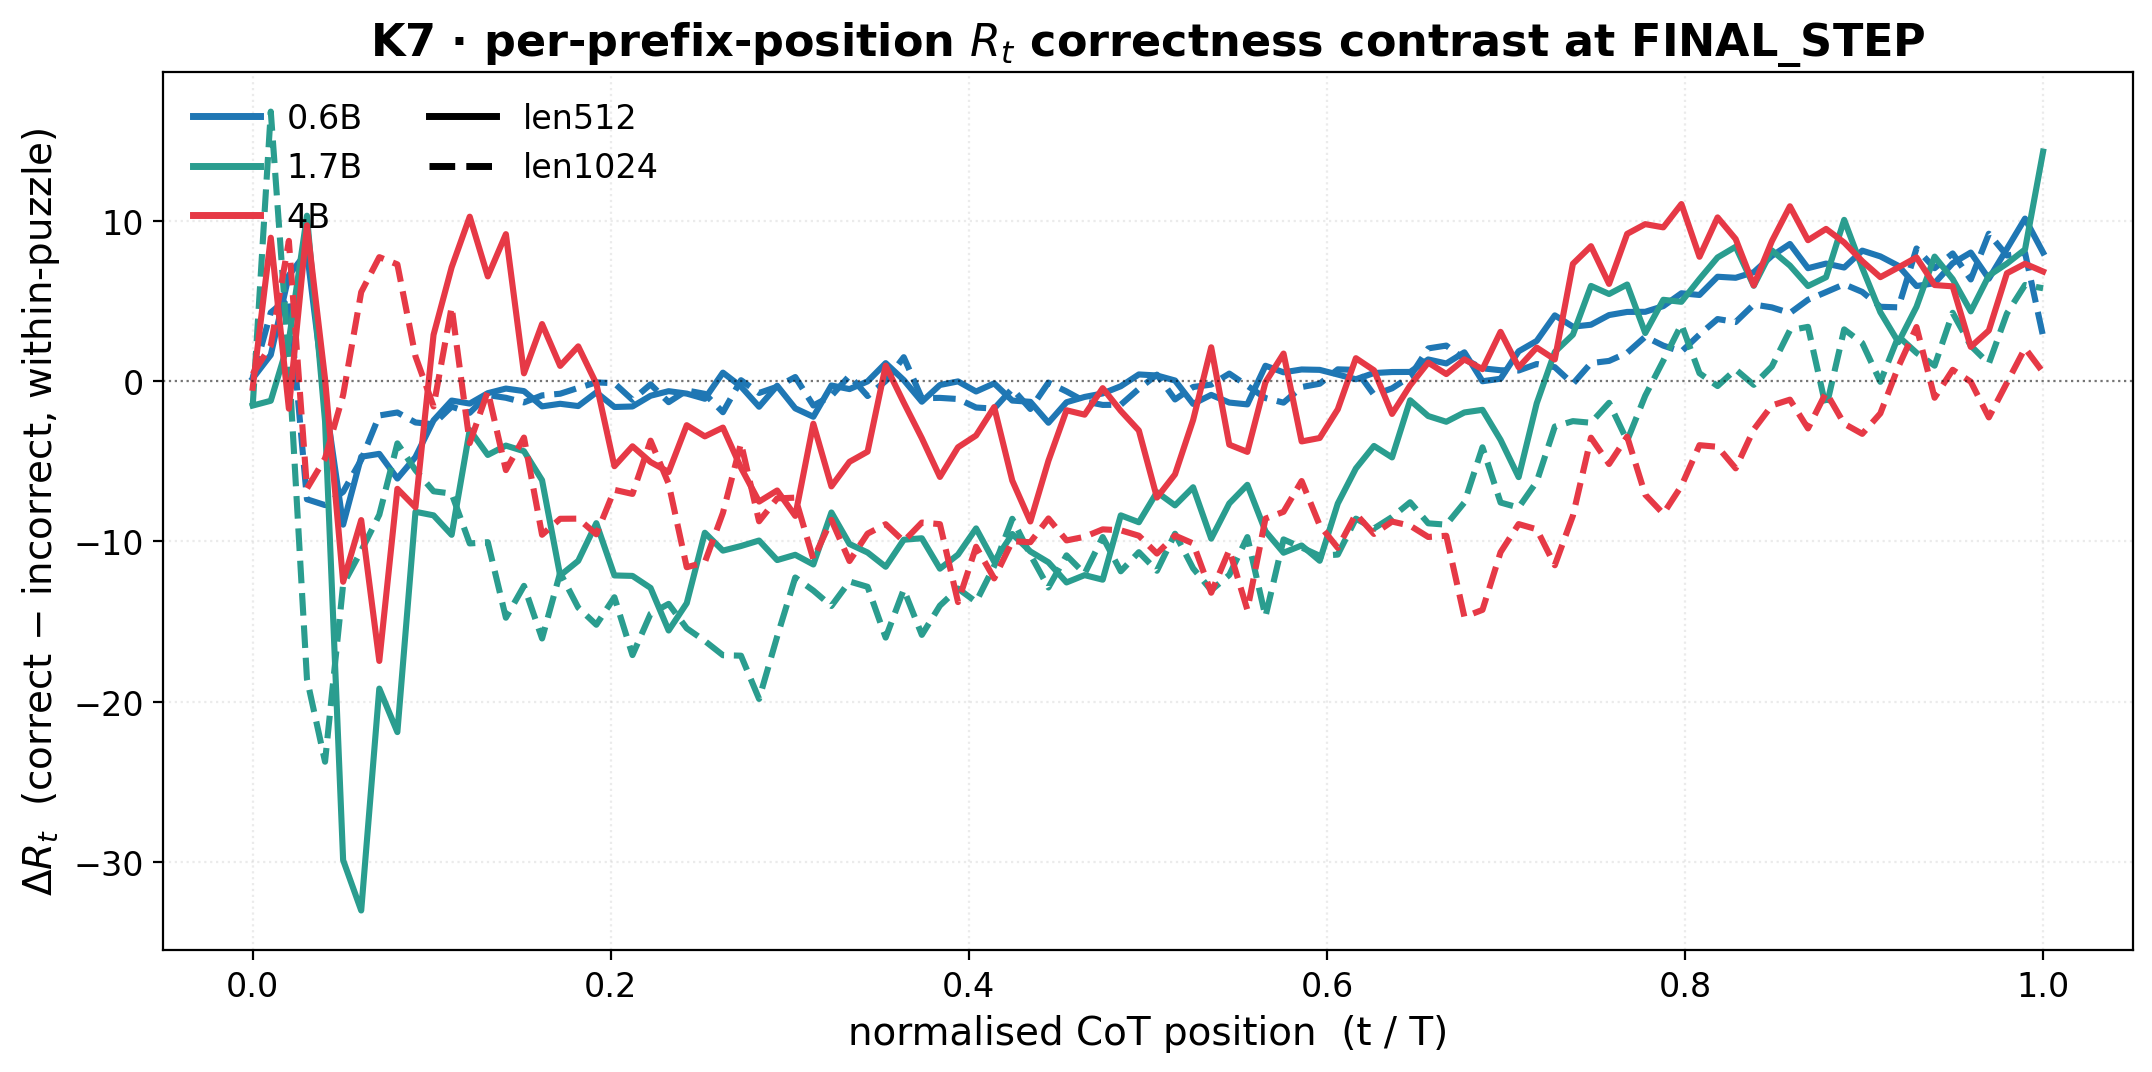
\includegraphics[width=0.85\linewidth]{figures/game24-k7.png}
  \caption{\textbf{K7 --- Per-prefix-position \(R_t\) correctness
  contrast at the final GRPO step.} Within-puzzle \(\Delta R_t\)
  averaged over puzzles with mixed correctness, one curve per
  (model, budget). Colour encodes model size, linestyle encodes
  budget; the dotted horizontal marks \(\Delta R_t = 0\).}
  \label{fig:k7}
\end{figure}

\paragraph{Summary.}
The baseline sweep documents (i) truncation-induced accuracy flattening
under a tight 512-token budget (K1), (ii) compaction of correct
rollouts with model scale even without
any length pressure (K2), (iii) latent diversity that shrinks as models
get stronger (K3), (iv) early saturation of solution coverage and
near-zero novelty by mid-training (K4), (v) high but scale-dependent
within-puzzle prefix collapse (K5), (vi) a usable but
competence-dependent \(R_T\) correctness contrast (K6), and (vii) a
late-CoT-dominated \(\Delta R_t\) trajectory whose early-position sign
flips track prefix collapse (K7). Sections
\ref{subsec:main-results}--\ref{subsec:diagnostics} will revisit each of
these panels under GRPO + predictive-velocity reward.

\subsection{Main Results}
\label{subsec:main-results}
\textit{TBD.} Accuracy and CoT-length curves over training steps for
baseline GRPO versus GRPO + predictive-velocity reward.

\subsection{Ablations}
\textit{TBD.} Effect of: (a)~the size and diversity of the reference-answer
set; (b)~replacing the velocity reward with the raw answer-prediction likelihood (to
confirm the camping problem); (c)~co-existence with length penalties (to
verify they become redundant).

\subsection{Diagnostics}
\label{subsec:diagnostics}
\textit{TBD.} Per-token reward attribution, redundancy measurements
(distinct-\(n\), self-BLEU on CoTs), and the zero-pass@\(K\) recovery
experiment.

\subsection{Setup}

\paragraph{Models and tasks.}
\textit{TBD.} Planned: Qwen3-1.7B / Qwen3-4B on GSM8K, with extensions to
MATH and a code-reasoning benchmark.

\paragraph{Baselines.}
We organise baselines in three groups, each isolating a different reason
the velocity reward might or might not help.

\textit{(A) Non-RL on correct trajectories.} These are the floor: do we
need RL at all, or does fine-tuning on correct rollouts suffice?
\begin{itemize}
  \item \textbf{SFT} on a fixed pool of canonical correct solutions.
  \item \textbf{Rejection-sampling fine-tuning} (RFT / ReST\textsuperscript{EM}~\citep{yuan2023rft, singh2023restem}):
        sample, filter by verifier, supervised fine-tune, repeat.
  \item \textbf{STaR}~\citep{zelikman2022star}: bootstrap rationales by
        SFT on filtered self-generated chains, with rationalisation on
        problems the model fails (the answer is revealed and a rationale
        is generated to match). This is the closest non-RL analogue to
        our prefix buffer \(\mathcal{P}_q\).
\end{itemize}

\textit{(B) RL with a sparse trajectory reward.} These isolate the value
of moving from trajectory-level to per-token credit.
\begin{itemize}
  \item \textbf{Vanilla GRPO}~\citep{shao2024deepseekmath, deepseek2025r1}
        with a verifiable correctness reward.
  \item \textbf{GRPO + linear length penalty}: \(R \leftarrow R - \lambda |o|\).
        The naive variant most practitioners try first; expected to trade
        accuracy for length.
  \item \textbf{GRPO + outcome-conditional length penalty} (Kimi-1.5
        style~\citep{kimi2025k15}): penalise length only on correct
        rollouts. The strongest hand-tuned baseline for D1; the one that
        could plausibly match the velocity reward's
        length--accuracy frontier.
\end{itemize}
For both penalised variants we report a sweep over \(\lambda\) and plot
the resulting (length, accuracy) Pareto curve, against which the
velocity-reward result is a single point.

\textit{(C) RL with a dense per-token reward.} These are the closest
competitors and isolate whether \emph{velocity-derived} density (change in
answer likelihood) is the right kind, as opposed to other analytic or
learned per-token signals.
\begin{itemize}
  \item \textbf{PRIME}~\citep{cui2025prime}: train an implicit process
        reward model with a DPO-style objective on outcome labels; its
        per-token log-ratio
        \(\beta\bigl[\log\pi_\phi(o_t \mid \cdot) - \log\pi_{\text{ref}}(o_t \mid \cdot)\bigr]\)
        is used as the dense RL signal. Like our velocity reward, the
        per-token decomposition is analytic; unlike ours, the signal
        measures policy-vs-reference deviation rather than change in
        the answer posterior.
  \item \textbf{PRM-guided PPO}~\citep{lightman2023letsverify, wang2024mathshepherd}:
        a learned step-level verifier supplies dense reward. Different
        mechanism (learned vs. analytic), same goal as PRIME and ours.
\end{itemize}

\paragraph{Implementation of \(r\) and \(v\).}
\textit{TBD.} We will detail how the reference answer \(a\) (or set of
equivalent answers) is sourced, how
\(\log p_\theta(a \mid q, o_{1:t})\) is evaluated (single masked forward
pass versus per-token recomputation), and how the velocity signal is
integrated with the GRPO group-relative baseline.

\bibliography{iclr2026_conference}
\bibliographystyle{iclr2026_conference}

\appendix
\section{Appendix}
\textit{Reserved for derivations, hyperparameters, and additional results.}

\subsection{Per-puzzle solution life-cycle across configs}
\label{app:lifecycle}

Figure~\ref{fig:lifecycle-grid} reproduces the lifecycle ``river'' of
\citet{shao2024deepseekmath}-style GRPO rollouts on a single held-out
Game-of-24 puzzle, drawn for every (model, budget) cell of the
\(\{0.6,1.7,4\}\)B \(\times\) \(\{512, 1024\}\) sweep. Each lane is one
unique AST-canonicalised expression; the thickness at training step
\(s\) equals the number of rollouts (out of \(G\)) that emitted that
expression that cycle, and the colour is green (verifier accepted) or
red (rejected). Comparing panels across rows isolates the effect of
model scale; across columns, the effect of the token budget.

\begin{figure}[h!]
  \centering
  \begin{subfigure}[t]{0.48\linewidth}
    \centering
    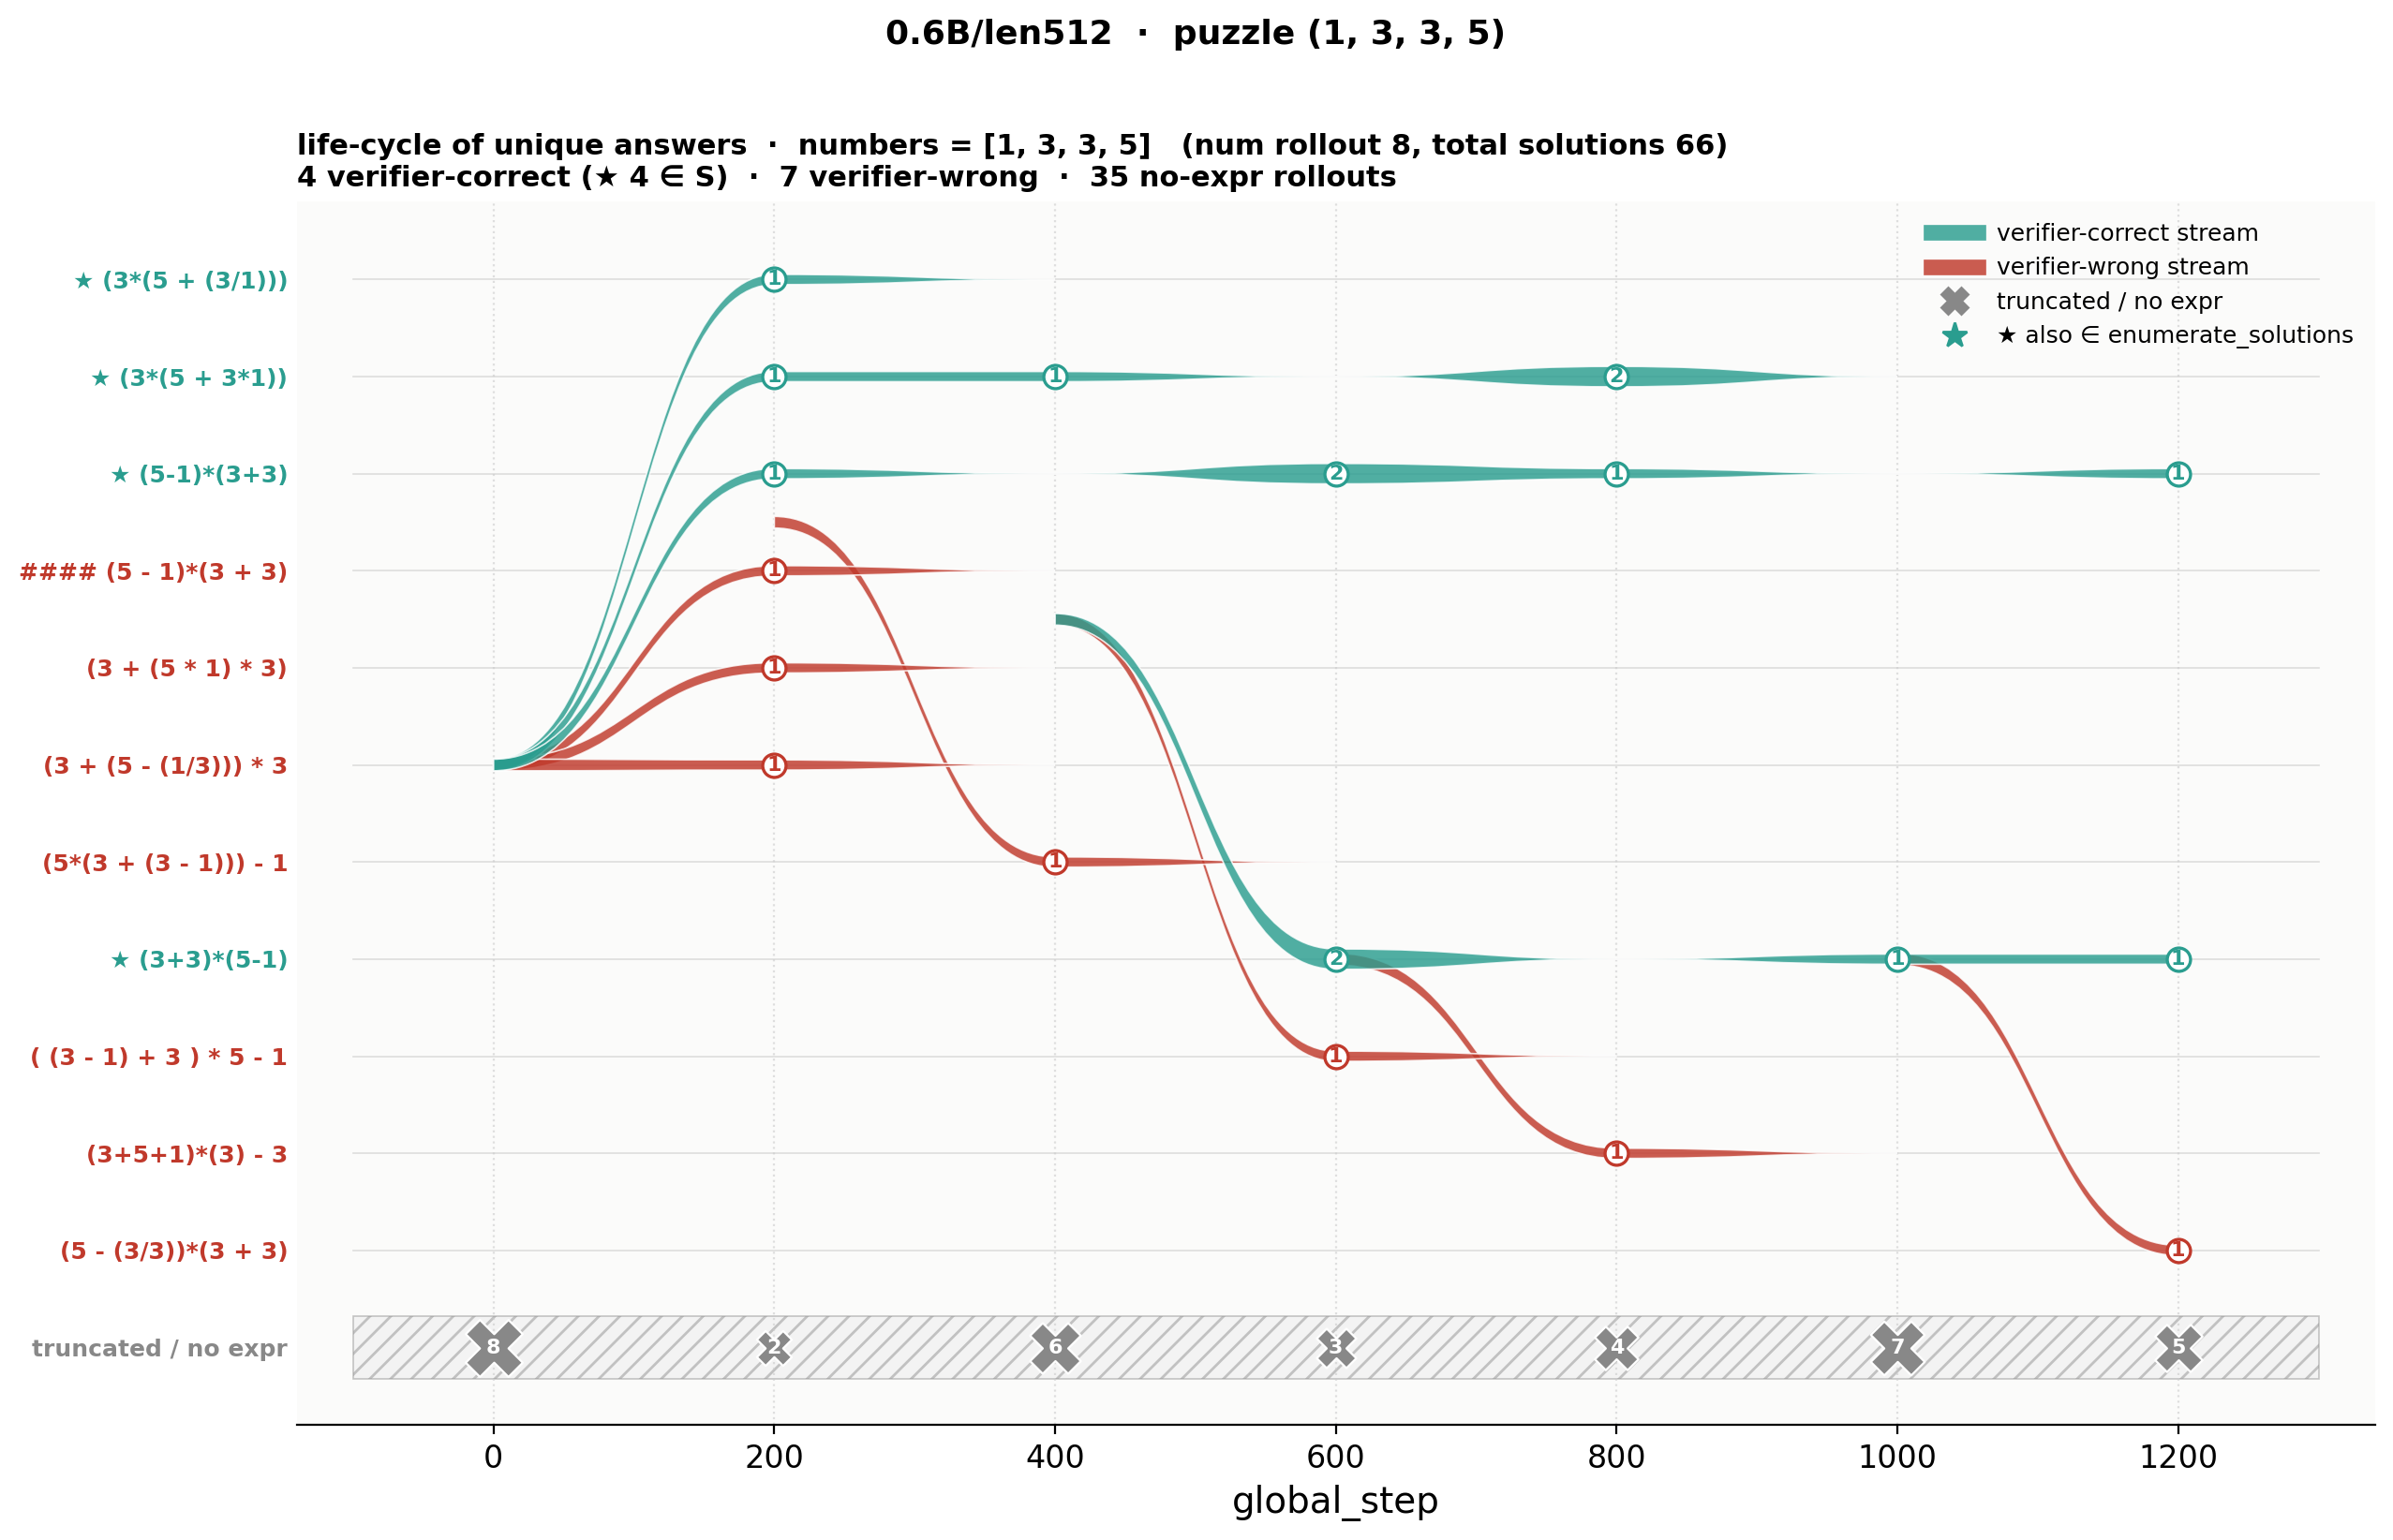
\includegraphics[width=\linewidth]{figures/game24-lifecycle-0.6B-len512.png}
    \caption{0.6B, \(T_{\max}=512\).}
  \end{subfigure}\hfill
  \begin{subfigure}[t]{0.48\linewidth}
    \centering
    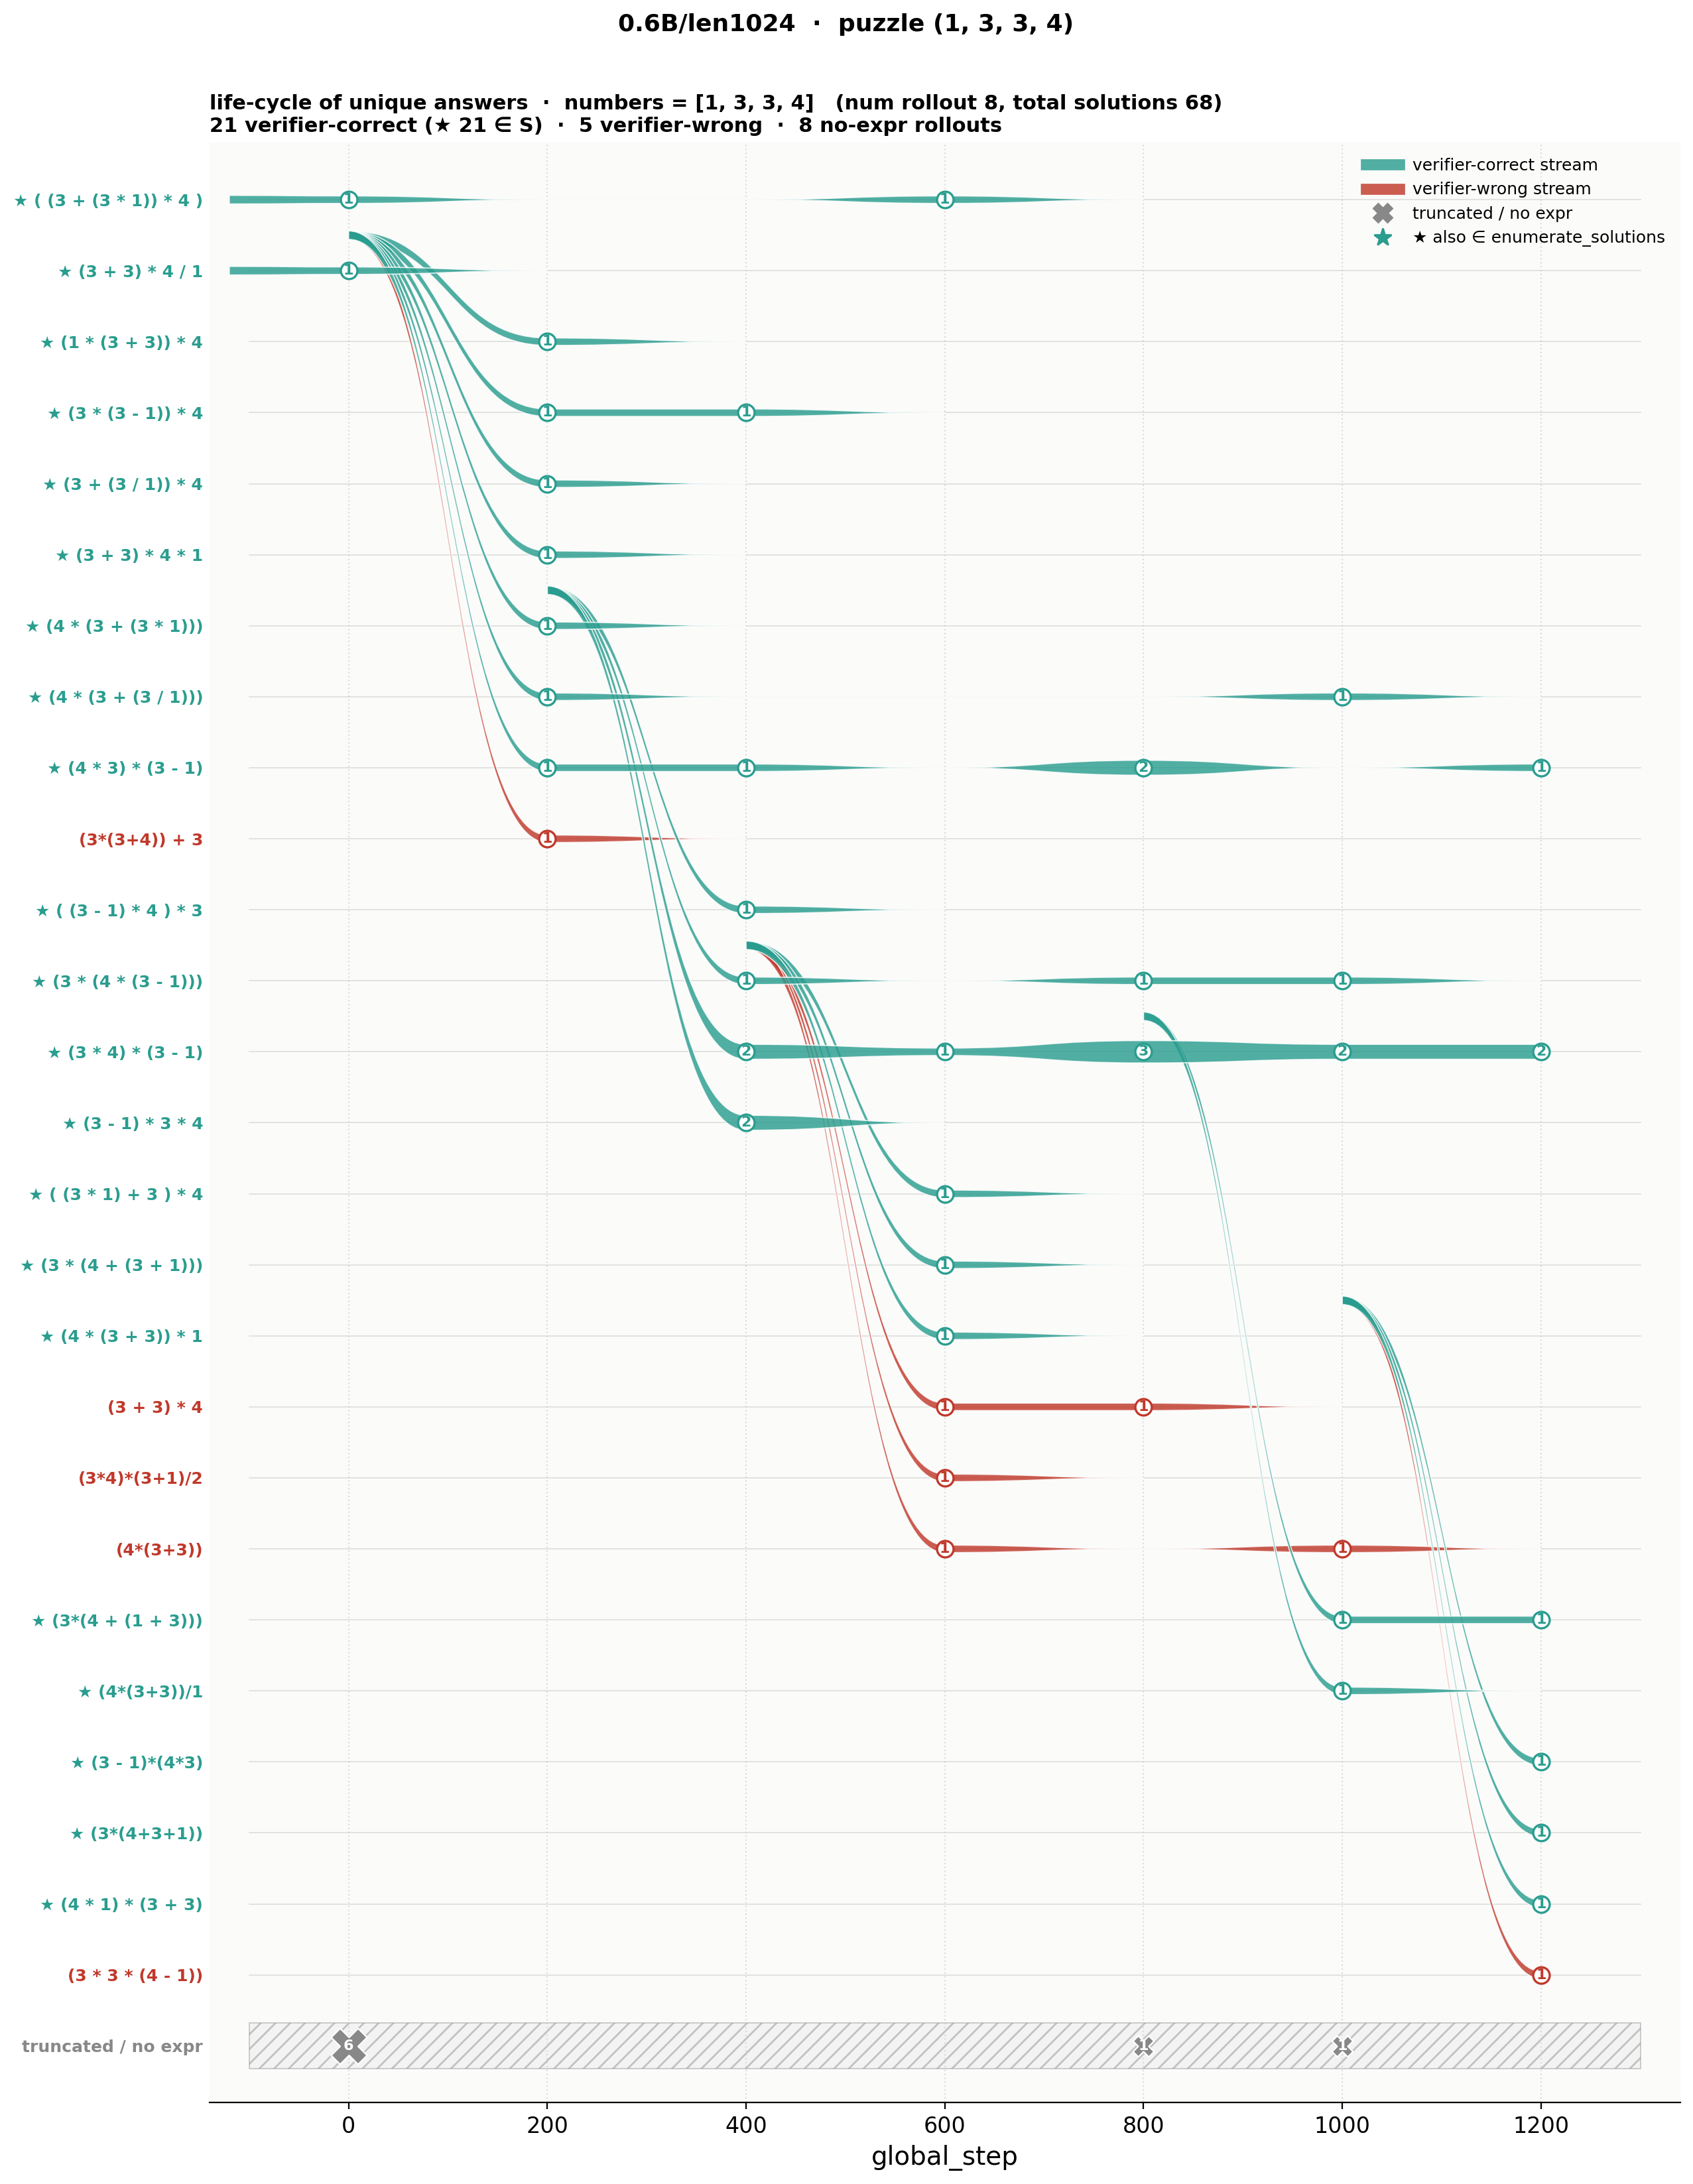
\includegraphics[width=\linewidth]{figures/game24-lifecycle-0.6B-len1024.png}
    \caption{0.6B, \(T_{\max}=1024\).}
  \end{subfigure}

  \vspace{0.6em}
  \begin{subfigure}[t]{0.48\linewidth}
    \centering
    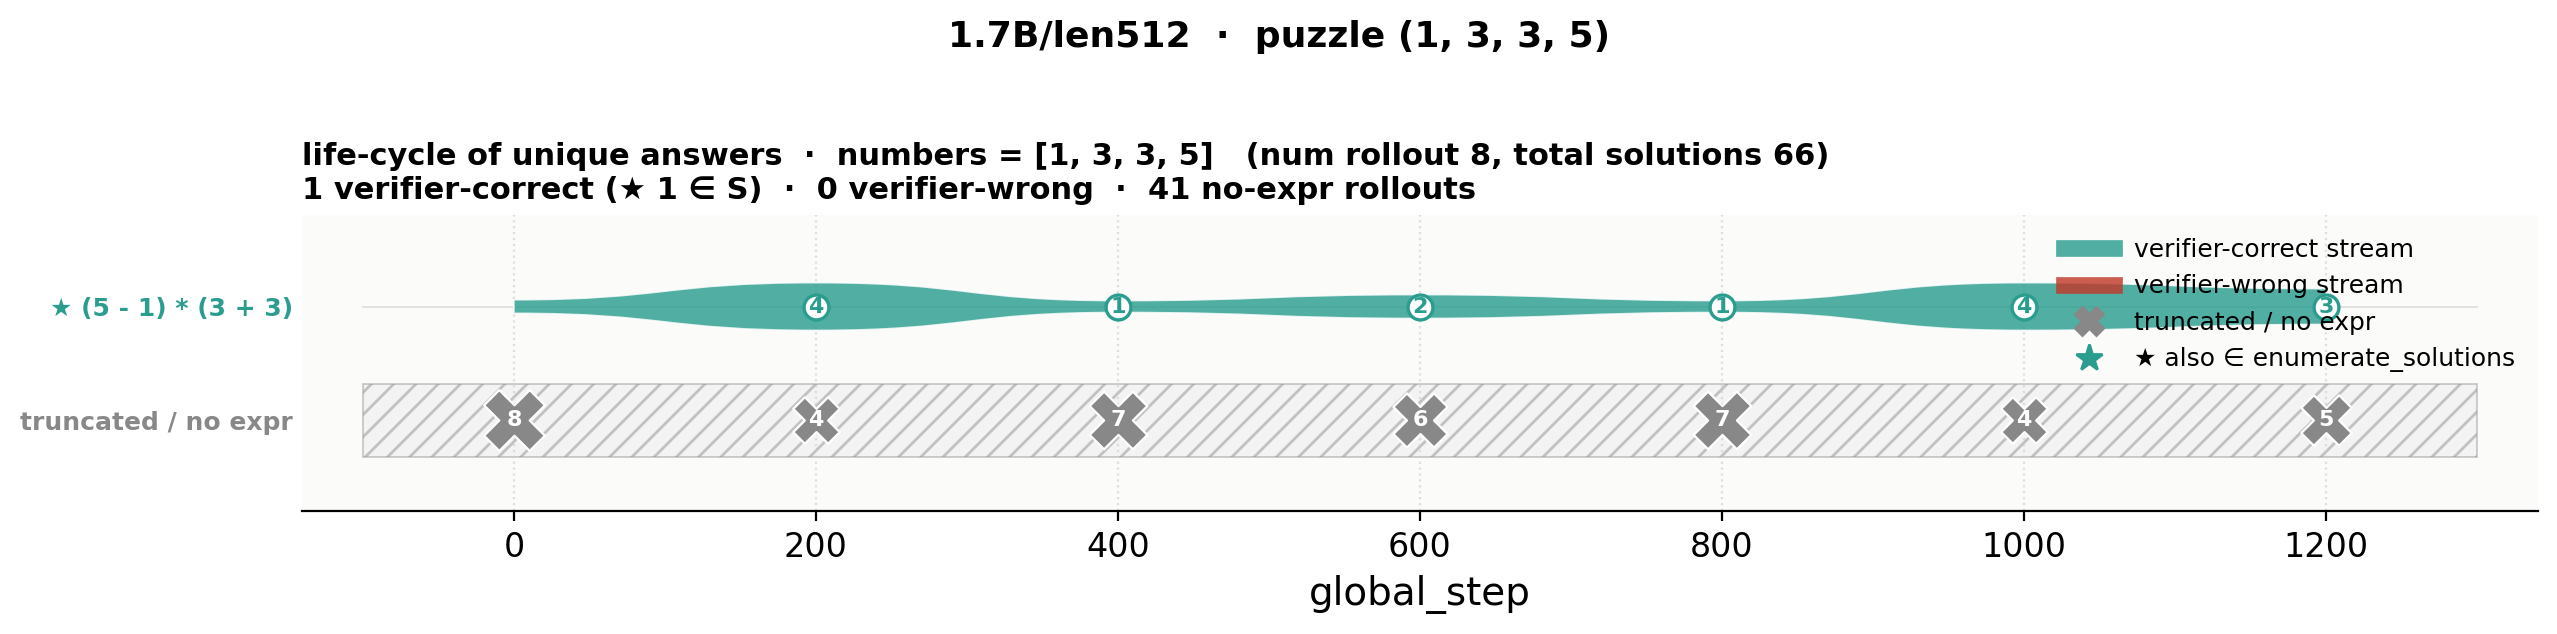
\includegraphics[width=\linewidth]{figures/game24-lifecycle-1.7B-len512.png}
    \caption{1.7B, \(T_{\max}=512\).}
  \end{subfigure}\hfill
  \begin{subfigure}[t]{0.48\linewidth}
    \centering
    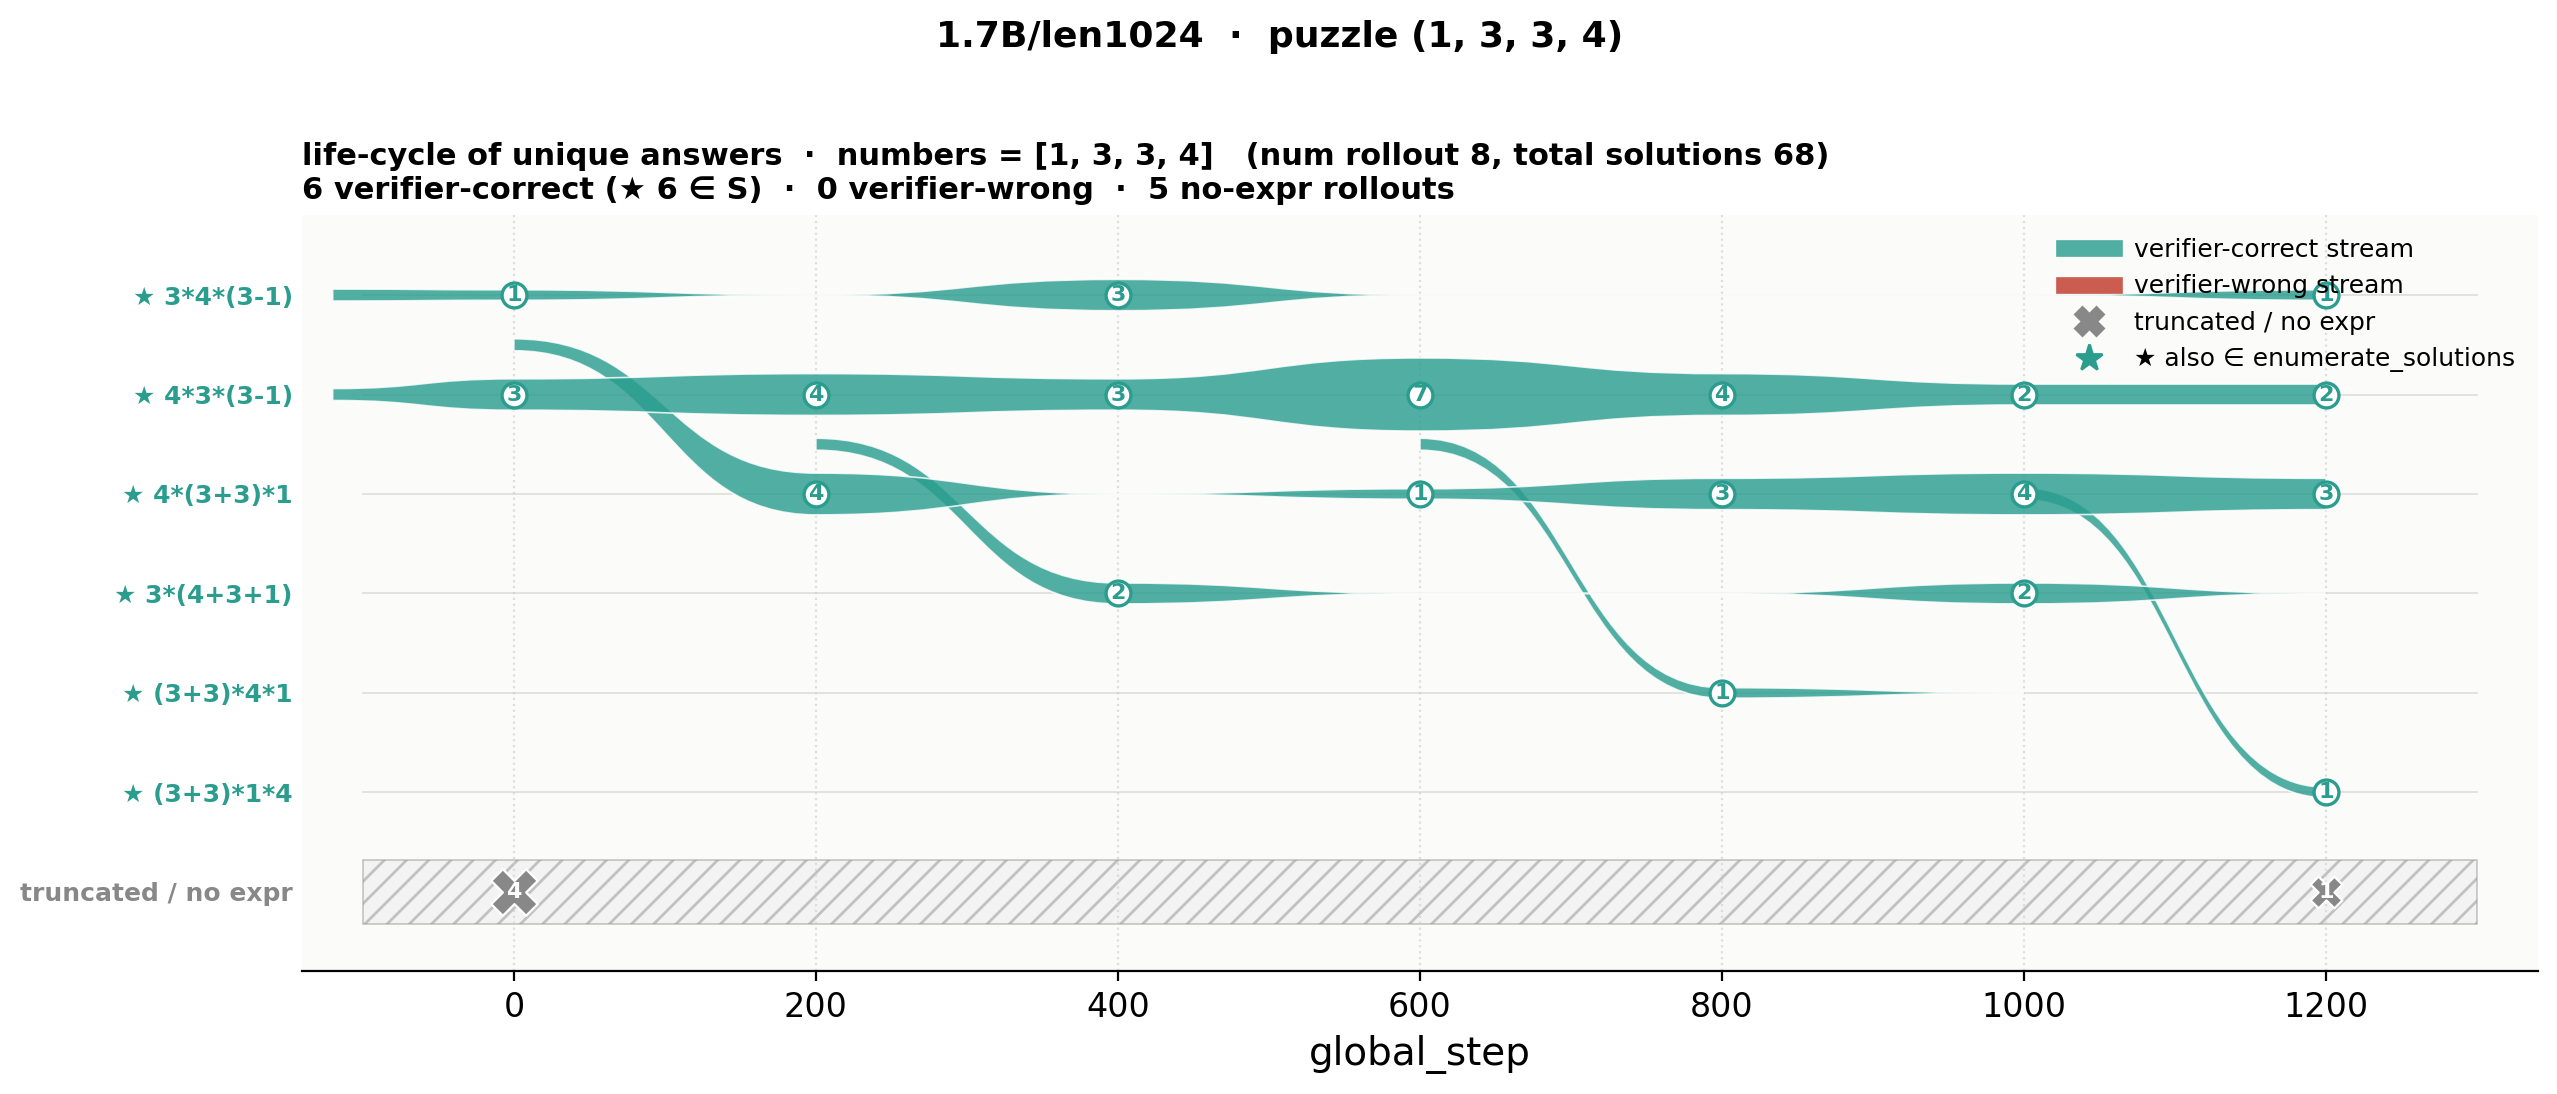
\includegraphics[width=\linewidth]{figures/game24-lifecycle-1.7B-len1024.png}
    \caption{1.7B, \(T_{\max}=1024\).}
  \end{subfigure}

  \vspace{0.6em}
  \begin{subfigure}[t]{0.48\linewidth}
    \centering
    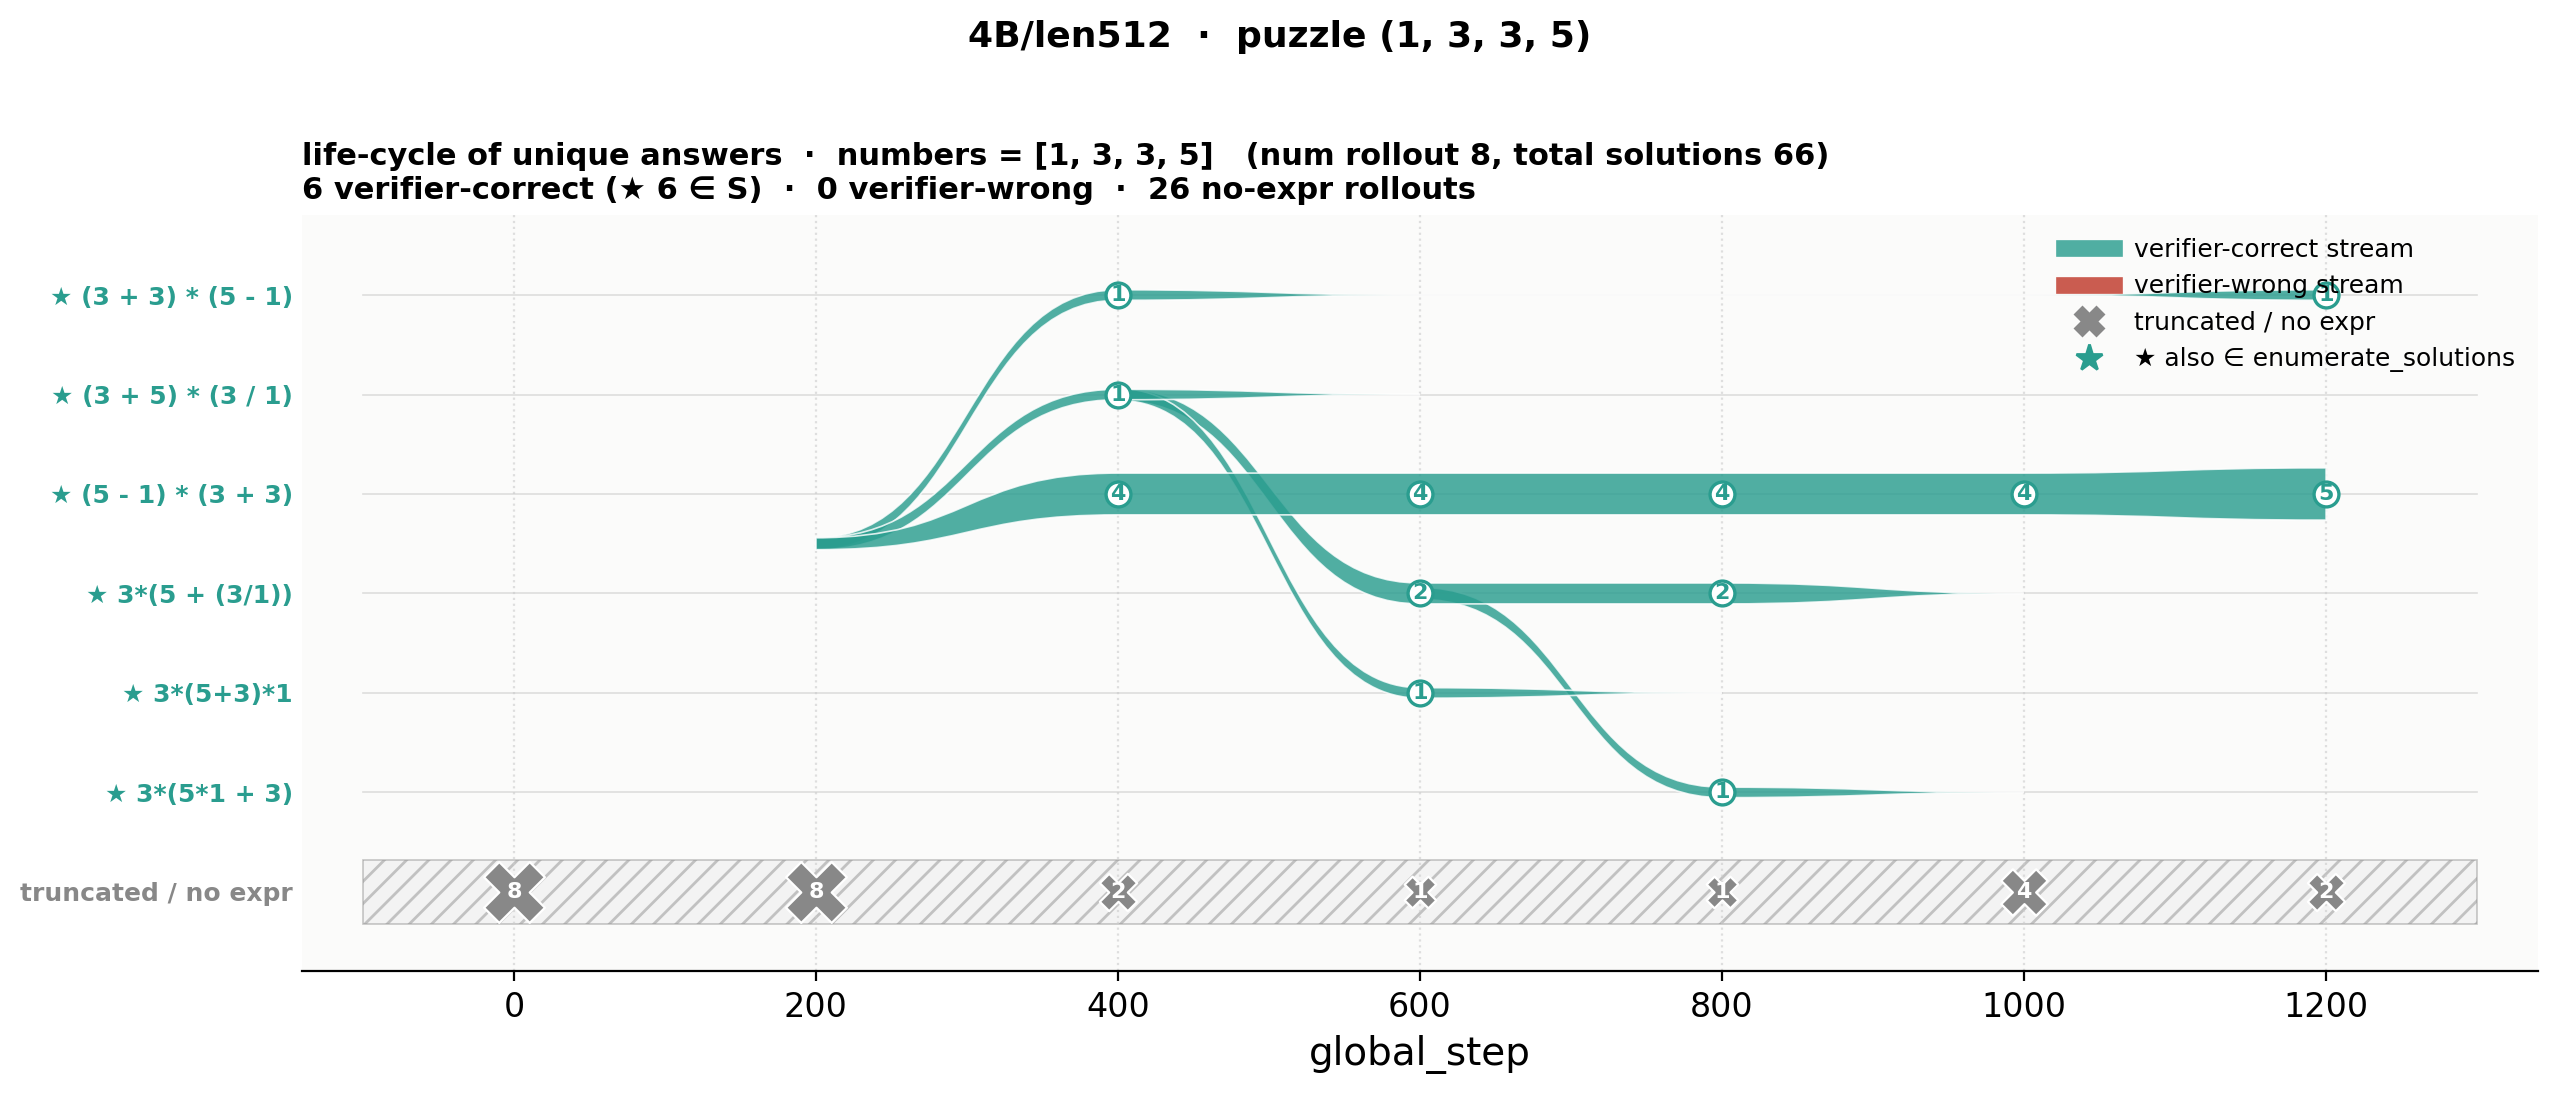
\includegraphics[width=\linewidth]{figures/game24-lifecycle-4B-len512.png}
    \caption{4B, \(T_{\max}=512\).}
  \end{subfigure}\hfill
  \begin{subfigure}[t]{0.48\linewidth}
    \centering
    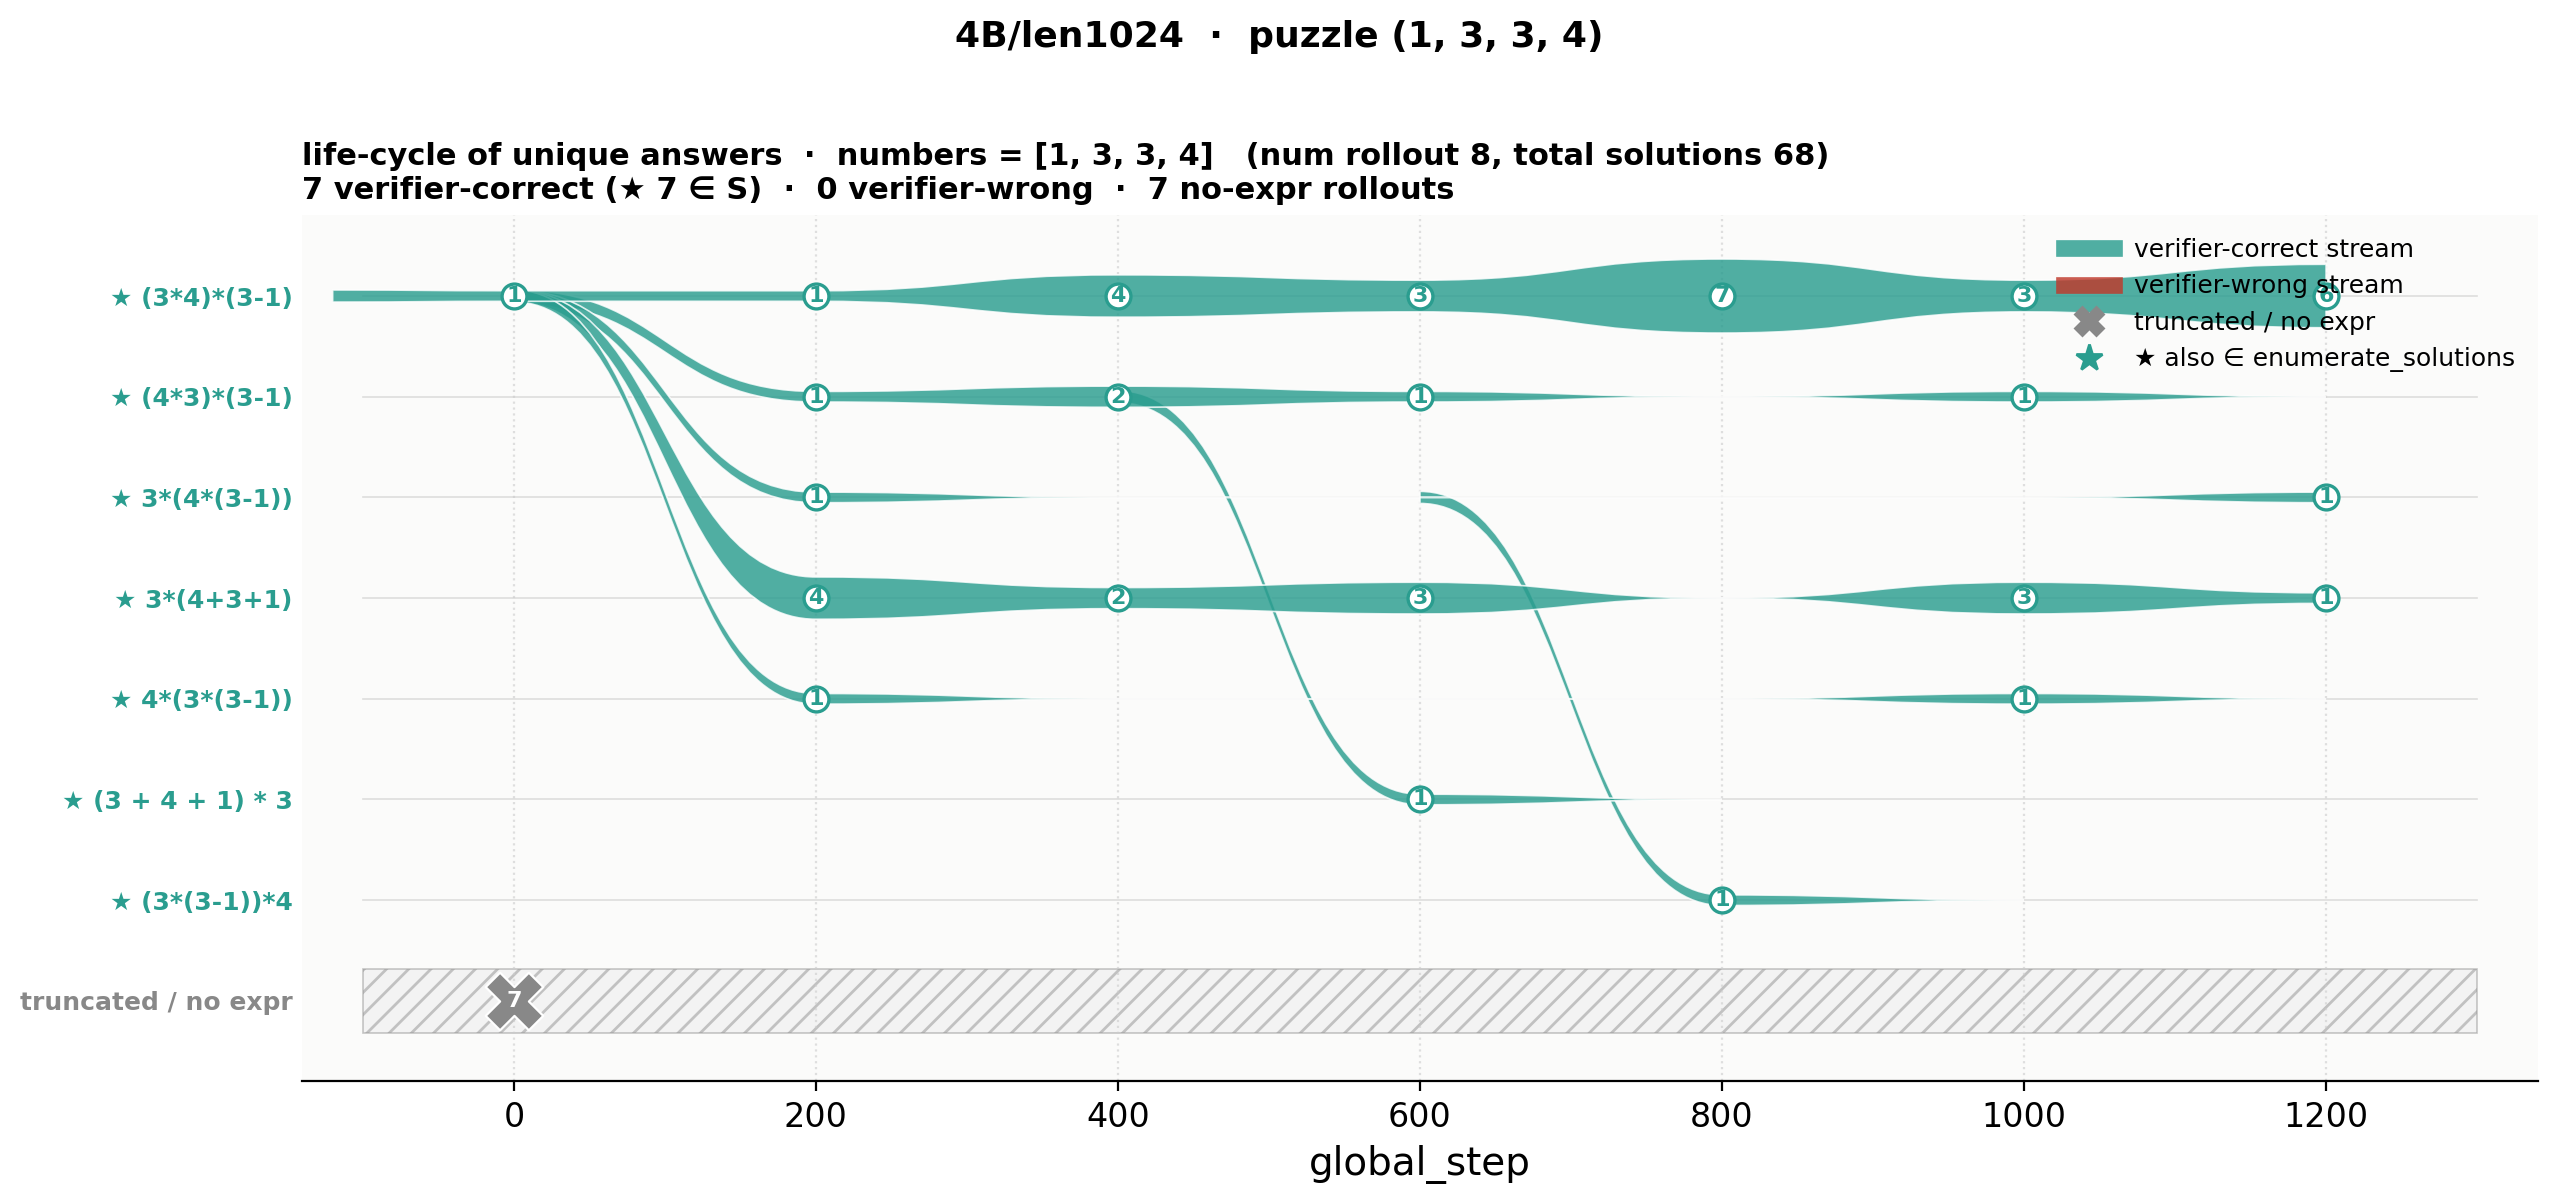
\includegraphics[width=\linewidth]{figures/game24-lifecycle-4B-len1024.png}
    \caption{4B, \(T_{\max}=1024\).}
  \end{subfigure}

  \caption{\textbf{Per-puzzle solution life-cycle across configs.}
  Stream graph of unique CoT/expressions emitted by vanilla GRPO over
  training, for one fixed held-out puzzle across the six
  (model, budget) cells.}
  \label{fig:lifecycle-grid}
\end{figure}

\end{document}
